\chapter{Predicción con imágenes modeladas}\label{cap.redes3dmod}

En este capítulo se presentan todos los estudios realizados en cuanto a la predicción en imágenes modeladas, con el objetivo de explorar distintas estructuras para atacar el problema. En particular, se quiere analizar el aporte de las redes recurrentes, que incorporan cierta memoria, a la solución.\\

En el mundo de las imágenes modeladas se ha afrontado la predicción como un problema de regresión, en el que la entrada es el conjunto de instantes de tiempo que se consideran conocidos (\textit{n}\_\textit{points}) con sus pares de posiciones (\textit{x}, \textit{y}) y la salida par de coordenadas en el instante de tiempo futuro. Cada una de estas coordenadas pueden tomar cualquier valor numérico decimal por lo que, como se explicó en la Sección~\ref{sec.eval}, es necesario realizar un redondeo para obtener la posición final, los píxeles están siempre representados por números enteros.\\

Para abordar la capacidad de predicción de las distintas redes propuestas se han utilizado los conjuntos generados, cuyas muestras siguen la estructura definida en la Figura~\ref{fig.dataset}, manteniendo fijos algunos parámetros:
\begin{itemize}
    \item El número de instantes temporales conocidos~(\textit{n}\_\textit{points}) es en todos los casos 20.
    \item La separación~(\textit{gap}) entre la última muestra conocida y la que se quiere predecir se establece en 10 instantes temporales.
    \item La división del conjunto se realiza con el 80\% de las muestras para el entrenamiento, el 10\% para validación, utilizado para el \textit{early stopping}, y el 10\% restante para el \textit{test}.
\end{itemize}

A continuación se realiza el recorrido por las distintas estructuras neuronales entrenadas, presentando los resultados obtenidos y las conclusiones que dan lugar a la exploración de distintas vías para la mejora de los mismos.

\section{Arquitectura no recurrente: Perceptrón Multicapa}
La primera aproximación para abordar la predicción de las imágenes modeladas considera una arquitectura de \acrshort{mlp} con una única capa oculta, explicado en detalle en el Apartado~\ref{ap.mlp}. En la Figura~\ref{fig.norec_simple_mod} se muestra un esquema que ilustra la arquitectura del \acrshort{mlp} utilizado para predecir la posición del píxel móvil en este formato de imagen. Esta estructura tiene como entrada 20 pares de valores (\textit{x}, \textit{y}) que alimentan una única capa oculta con 10 neuronas, proporcionando a la salida un par de valores que se corresponde con la posición estimada.\\

\begin{figure}[H]
		\begin{center}
			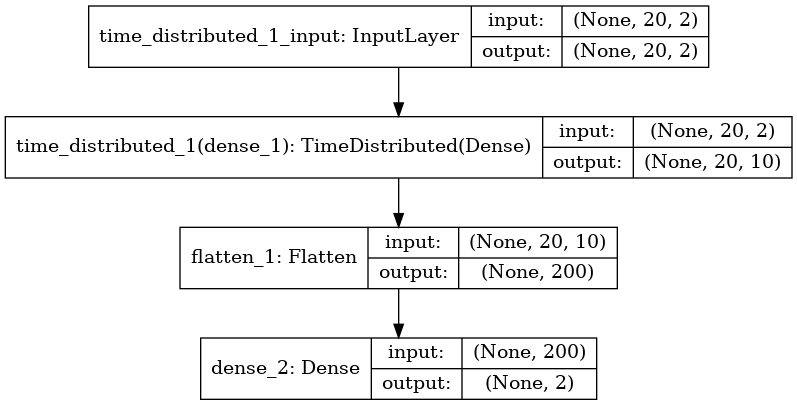
\includegraphics[width=0.8\textwidth]{ figures/net/NOREC_simple_mod.png}
			\caption{Estructura de \acrshort{mlp} con 1 capa oculta y 10 neuronas para imágenes modeladas.}
			\label{fig.norec_simple_mod}
		\end{center}
\end{figure}
\vspace{-10pt}

Tras la definición de la red, se realizan diversos experimentos con el objetivo de lograr la predicción en el escenario más complejo considerado. Se aumenta de forma progresiva la complejidad en el movimiento, considerando en primera instancia más grados de libertad, y posteriormente otras dinámicas.

\subsection{Influencia del número muestras}\label{ap.muestras}
Antes de comenzar con el estudio de las distintas redes con las dinámicas consideradas se realiza un breve estudio sobre el número de muestras utilizando el caso especial de la dinámica lineal, con pendiente nula, por su sencillez. Bajo esta premisa, se emplea en primer lugar un conjunto de 1000 muestras, de las cuales 800 se emplean para entrenamiento, 100 para validación y las 100 restantes para \textit{test}.\\

En la Figura~\ref{fig.norec_urm_fix_1000} se muestran los resultados obtenidos al evaluar la red entrenada con el conjunto cuya altura inicial del píxel en la imagen permanece fija.

\begin{figure}[H]
		\begin{center}
			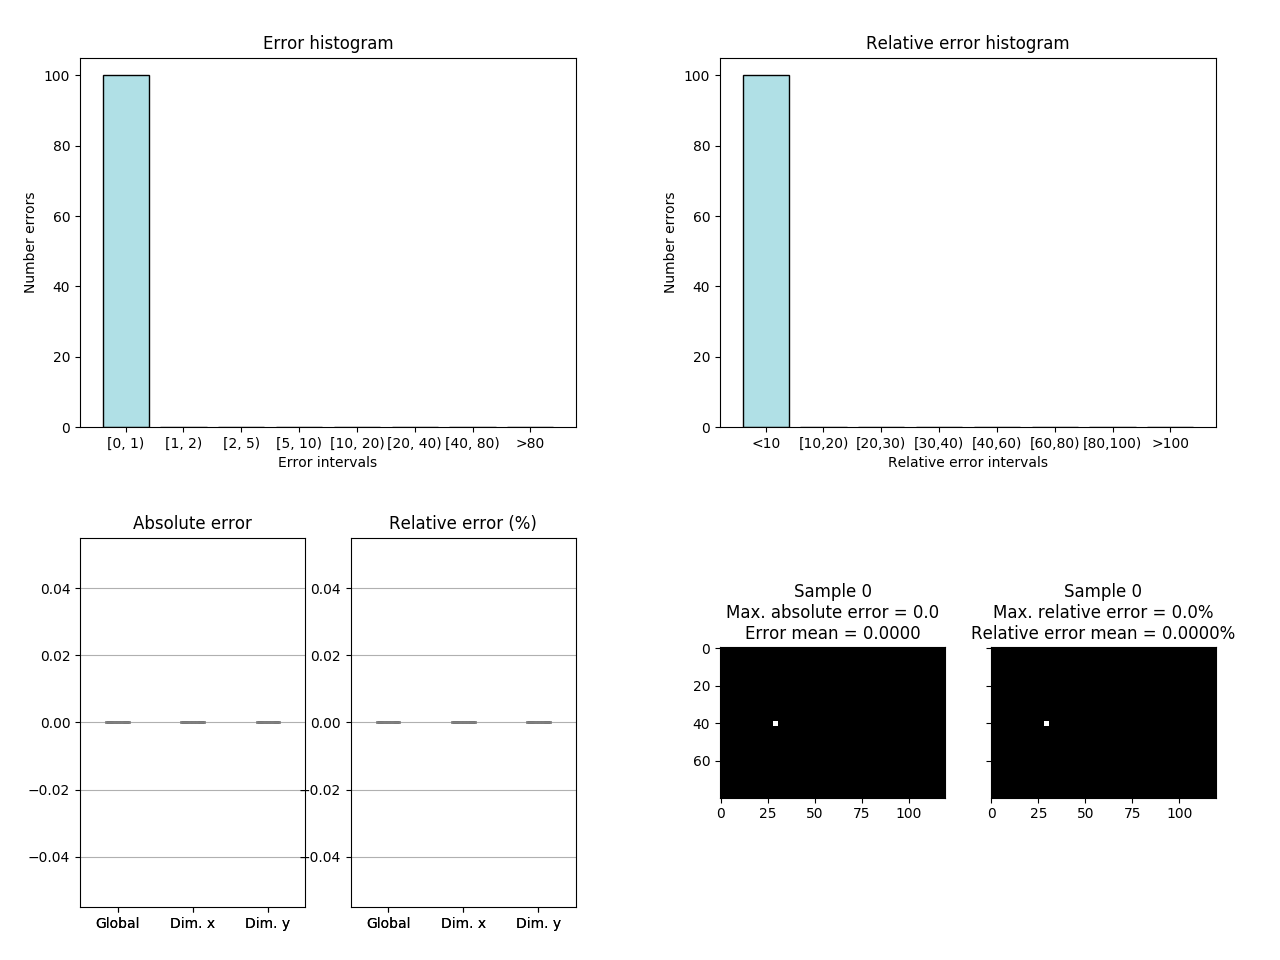
\includegraphics[width=0.8\textwidth]{ figures/test_mod/NOREC/URM_fix_1000.png}
			\caption{Resultados de \acrshort{mlp} con dinámica lineal, pendiente nula y altura fija en imágenes modeladas~(100 muestras de \textit{test})}
			\label{fig.norec_urm_fix_1000}
		\end{center}
\end{figure}
\vspace{-10pt}

El error obtenido en este caso es nulo ya que, al mantener fija la altura y aplicar las restricciones de aparición del píxel en todas la imágenes, el número de muestras distintas es mucho menor a las 1000 creadas. Este hecho hace que la red aprenda todos los ejemplos posibles en el entrenamiento, evitando que se pueda equivocar en cualquiera de los ejemplos de \textit{test}.\\

Con el objetivo de incrementar la complejidad de la dinámica, se entrena la misma estructura de red con el mismo número de muestras pero dejando la altura inicial como parámetro libre en cada predicción. Los resultados de la evaluación de esta nueva red, que se muestran en la Figura~\ref{fig.norec_urm_var_1000}, ya no son tan buenos como en el caso anterior. La razón es que, al dejar que la altura inicial tome un valor aleatorio ha aumentado la variabilidad de las muestras, impidiendo que la red vea la totalidad de las variantes en la fase de entrenamiento, presentando casos desconocidos en la evaluación.

\begin{figure}[H]
		\begin{center}
			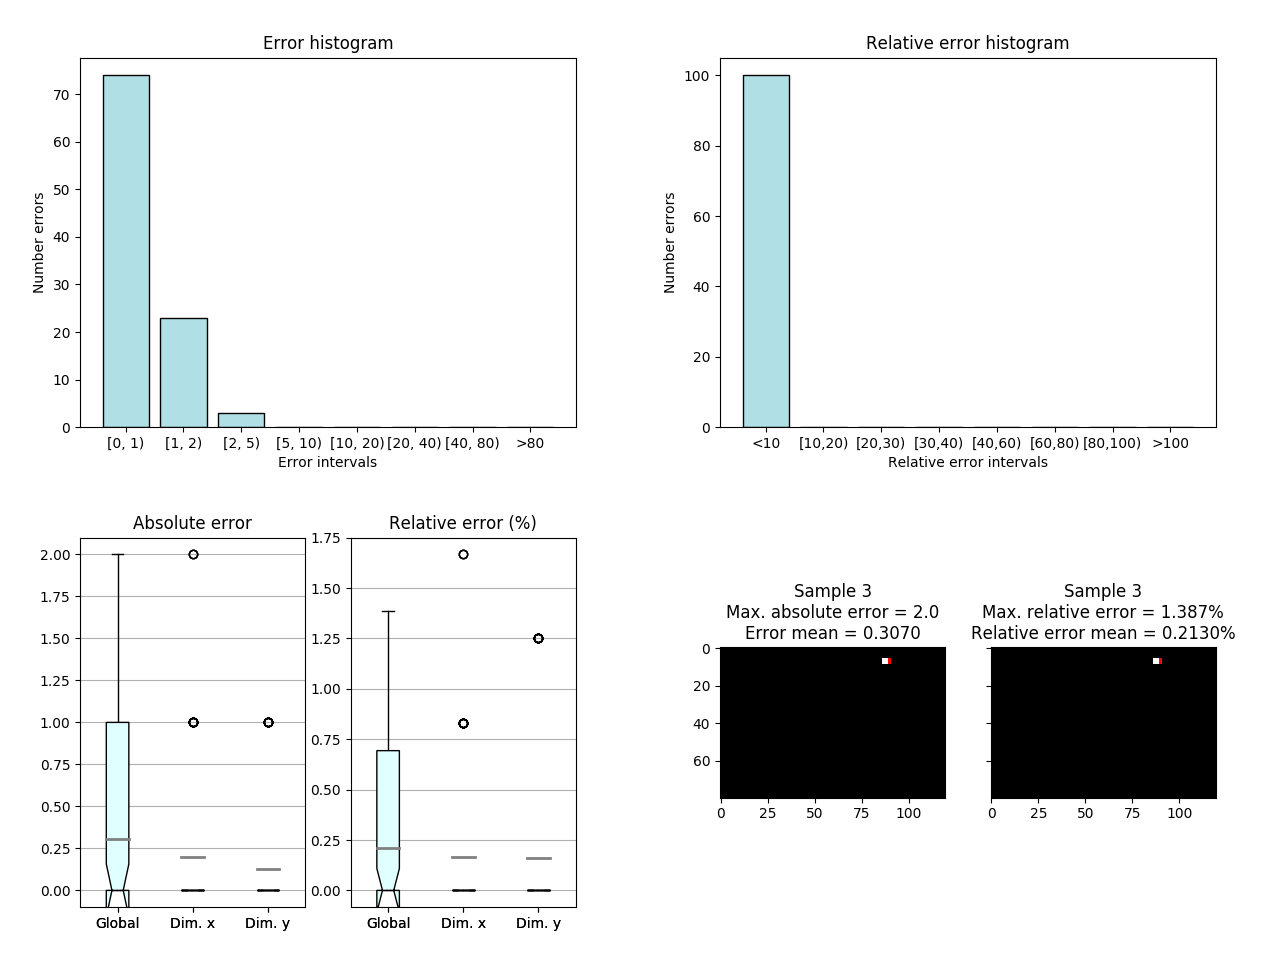
\includegraphics[width=0.8\textwidth]{ figures/test_mod/NOREC/URM_var_1000.png}
			\caption{Resultados de \acrshort{mlp} con dinámica lineal, pendiente nula y altura aleatoria en imágenes modeladas~(100 muestras de \textit{test}).}
			\label{fig.norec_urm_var_1000}
		\end{center}
\end{figure}
\vspace{-10pt}

La primera acción  para tratar de mejorar los resultados es aumentar el número de muestras para incrementar el número de ejemplos de los que la red aprende. En esta línea, se genera un nuevo conjunto de 5000 muestras con la misma proporción en la generación de las tres particiones: 4000 destinadas al entrenamiento, 500 a la validación y otras 500 al \textit{test}. Los resultados de la red entrenada con este nuevo conjunto se muestran en la Figura~\ref{fig.norec_urm_var_5000}, en la que se puede comprobar que el error vuelve a ser nulo.

\begin{figure}[H]
		\begin{center}
			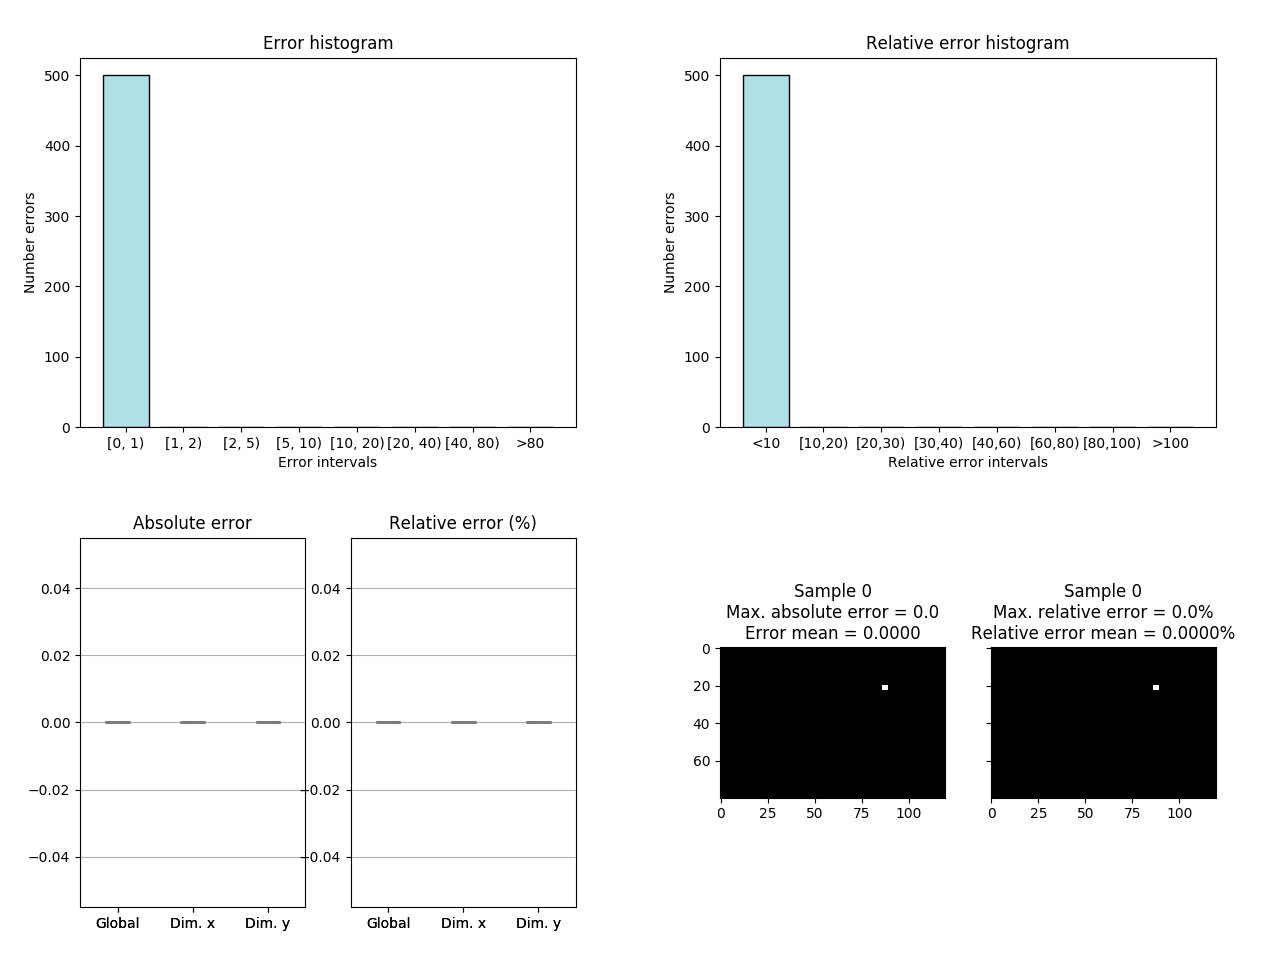
\includegraphics[width=0.8\textwidth]{ figures/test_mod/NOREC/URM_var_5000.png}
			\caption{Resultados de \acrshort{mlp} con dinámica lineal, pendiente nula y altura fija en imágenes modeladas~(500 muestras de \textit{test}).}
			\label{fig.norec_urm_var_5000}
		\end{center}
\end{figure}
\vspace{-10pt}

Con los resultados obtenidos se concluye que utilizar un mayor número de muestras es un factor que hace mejorar los resultados, pues la red aprende de una mayor variedad de ejemplos. Sin embargo, cuando se obtiene un acierto del 100\%, como en el primer caso, no hay margen de mejora y únicamente se consigue aumentar la complejidad computacional. Es decir, el aumento de muestras es un factor de mejora siempre que la naturaleza de las mismas sea lo suficientemente compleja como para necesitar un mayor número de observaciones para modelar la estadística subyacente en los datos.

\subsection{Predicción con dinámicas lineales}
Para abordar la predicción de fotogramas que representan objetos siguen una dinámica lineal se emplea un conjunto con un total de 10000 muestras dividido en 8000 muestras para entrenamiento, 1000 para validación y 1000 para evaluación.\\

En primer lugar se realiza el estudio de esta dinámica con un único \acrshort{dof}, la pendiente de la trayectoria del píxel activo, cuyos resultados de evaluación de la red entrenada queda reflejado en la Figura~\ref{fig.norec_lin_fix_10000}.

\begin{figure}[H]
		\begin{center}
			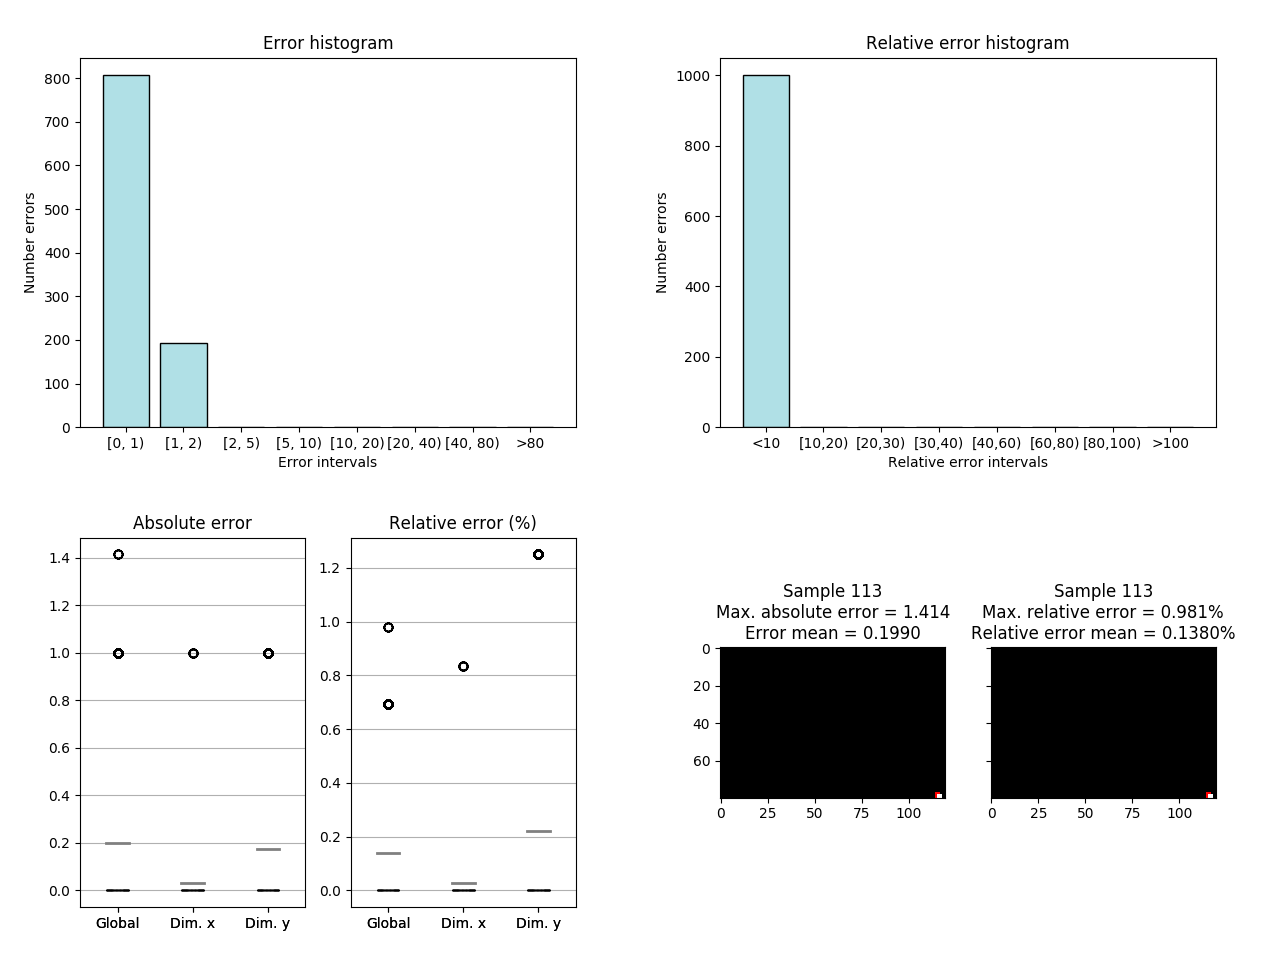
\includegraphics[width=0.8\textwidth]{ figures/test_mod/NOREC/linear_fix_10000.png}
			\caption{Resultados de \acrshort{mlp} con dinámica lineal de 1 \acrshort{dof} en imágenes modeladas~(1000 muestras de \textit{test}).} 
			\label{fig.norec_lin_fix_10000}
		\end{center}
\end{figure}
\vspace{-10pt}

Se puede comprobar que la capacidad de predicción de esta red es buena, ofreciendo un error relativo muy reducido tanto en términos de media como de máximo.\\

Se aumenta el grado de complejidad de la dinámica con un nuevo \acrshort{dof}, la altura inicial, y se repite el experimento con la misma estructura de red, cuyos resultados se reflejan en la Figura~\ref{fig.norec_lin_var_10000}. Como era de esperar, dejar mayor libertad de movimiento al píxel activo, aumentando la complejidad, repercute de forma directa en la capacidad de predicción de la red. Sin embargo, los resultados obtenidos indican que la red continúa siendo capaz de predecir bien bajo estas condiciones.\\

Dados los resultados para el caso más complejo de la dinámica lineal, 2~\acrshort{dof}, se concluye que, con el número de muestras modeladas establecidas y la estructura de red propuesta, es posible predecir satisfactoriamente la posición de un píxel móvil que sigue una dinámica lineal, independientemente de sus \acrshort{dof}.

\begin{figure}[H]
		\begin{center}
			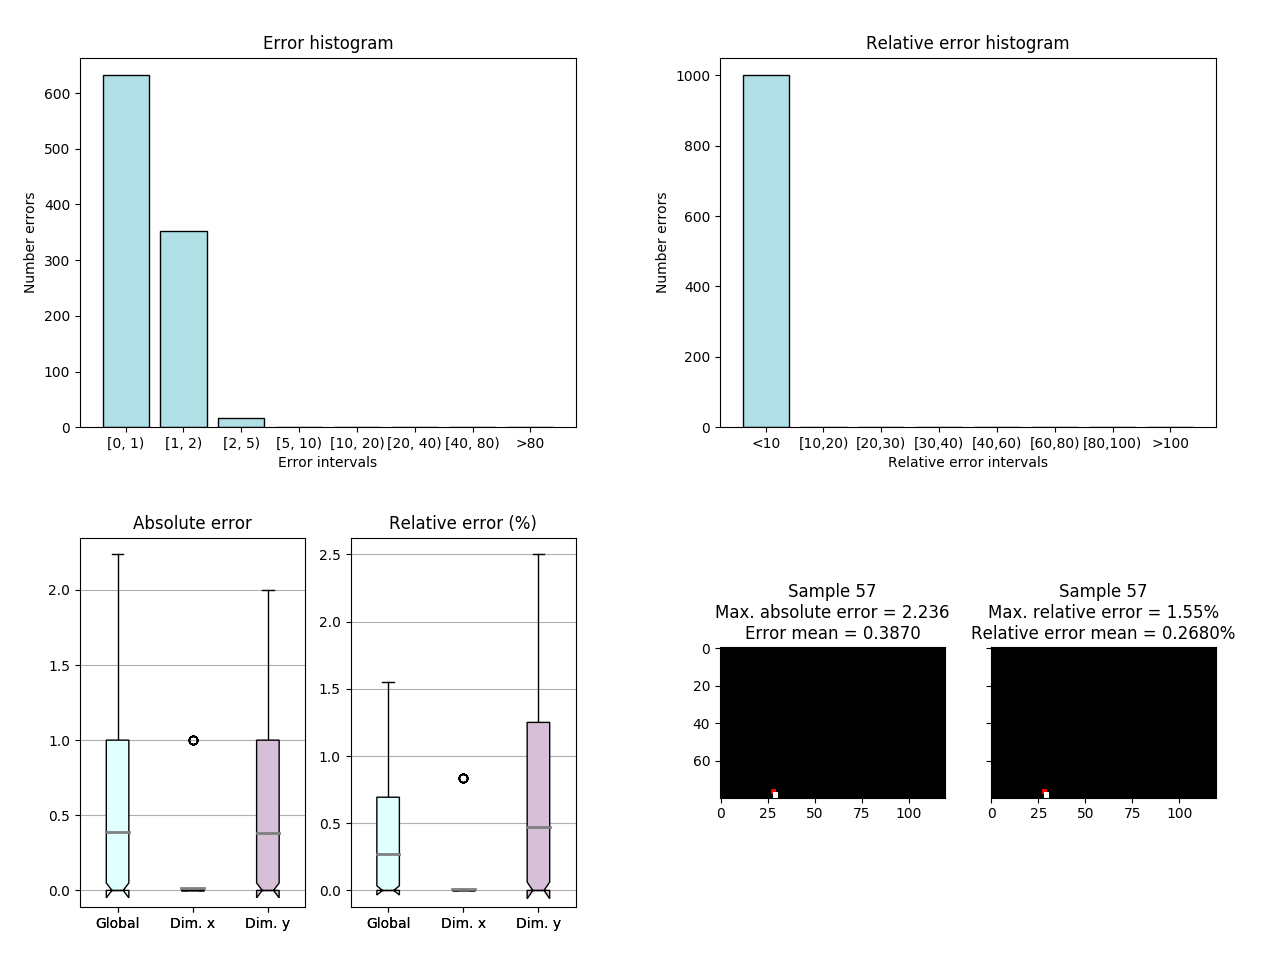
\includegraphics[width=0.8\textwidth]{ figures/test_mod/NOREC/linear_var_10000.png}
			\caption{Resultados de \acrshort{mlp} con dinámica lineal de 2 \acrshort{dof} en imágenes modeladas~(1000 muestras de \textit{test}).}
			\label{fig.norec_lin_var_10000}
		\end{center}
\end{figure}
\vspace{-10pt}


\subsection{Predicción con dinámicas parabólicas}
Para abordar la predicción de fotogramas que representan objetos siguen una dinámica parabólica se utiliza un conjunto con 10000 ejemplos, divididos de la misma manera que en la dinámica anterior.\\

El análisis de la capacidad predictiva de la red comienza con el caso más sencillo,  un único \acrshort{dof}, el valor de \textit{a} en esta dinámica. La Figura~\ref{fig.norec_parab_fix_10000} muestra los resultados obtenidos al evaluar la red entrenada bajo estas condiciones. Estos resultados demuestran que la red propuesta es capaz de predecir bien la posición del píxel móvil en este primer caso.

\begin{figure}[H]
		\begin{center}
			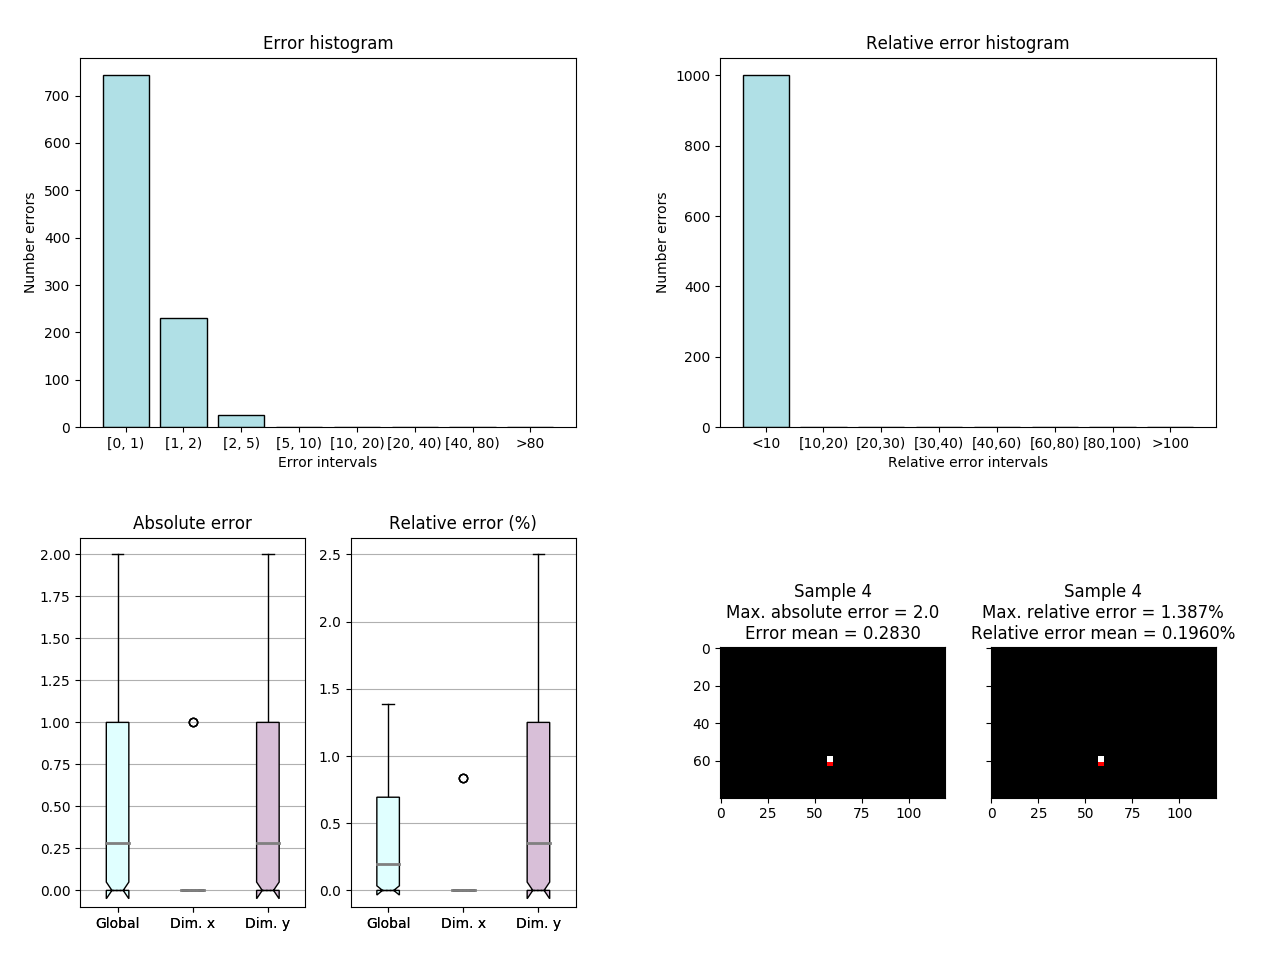
\includegraphics[width=0.8\textwidth]{ figures/test_mod/NOREC/parab_fix_10000.png}
			\caption{Resultados de \acrshort{mlp} con dinámica parabólica de 1 \acrshort{dof} en imágenes modeladas~(1000 muestras de \textit{test}).} 
			\label{fig.norec_parab_fix_10000}
		\end{center}
\end{figure}
\vspace{-10pt}

Tras los buenos resultados obtenidos con el primer caso de la dinámica, 1~\acrshort{dof},se prosigue con el aumento del los \acrshort{dof} para poner a prueba la estructura.\\

En las Figuras~\ref{fig.norec_parab_var_10000}~y~\ref{fig.norec_parab_var1_10000} se muestran los resultados obtenidos para las predicción de la dinámica con 2 y 3 \acrshort{dof}, la altura inicial y \textit{c}, respectivamente. A la vista de estos resultados se comprueba que, a pesar de que los resultados empeoran ligeramente al introducir más grados de libertad, éste se mantiene en unos valores razonables. Se concluye que, para imágenes modeladas, el \acrshort{mlp} es capaz de predecir el desplazamiento del píxel según la dinámica parabólica, independientemente del nivel de complejidad que se establezca.

\begin{figure}[H]
		\begin{center}
			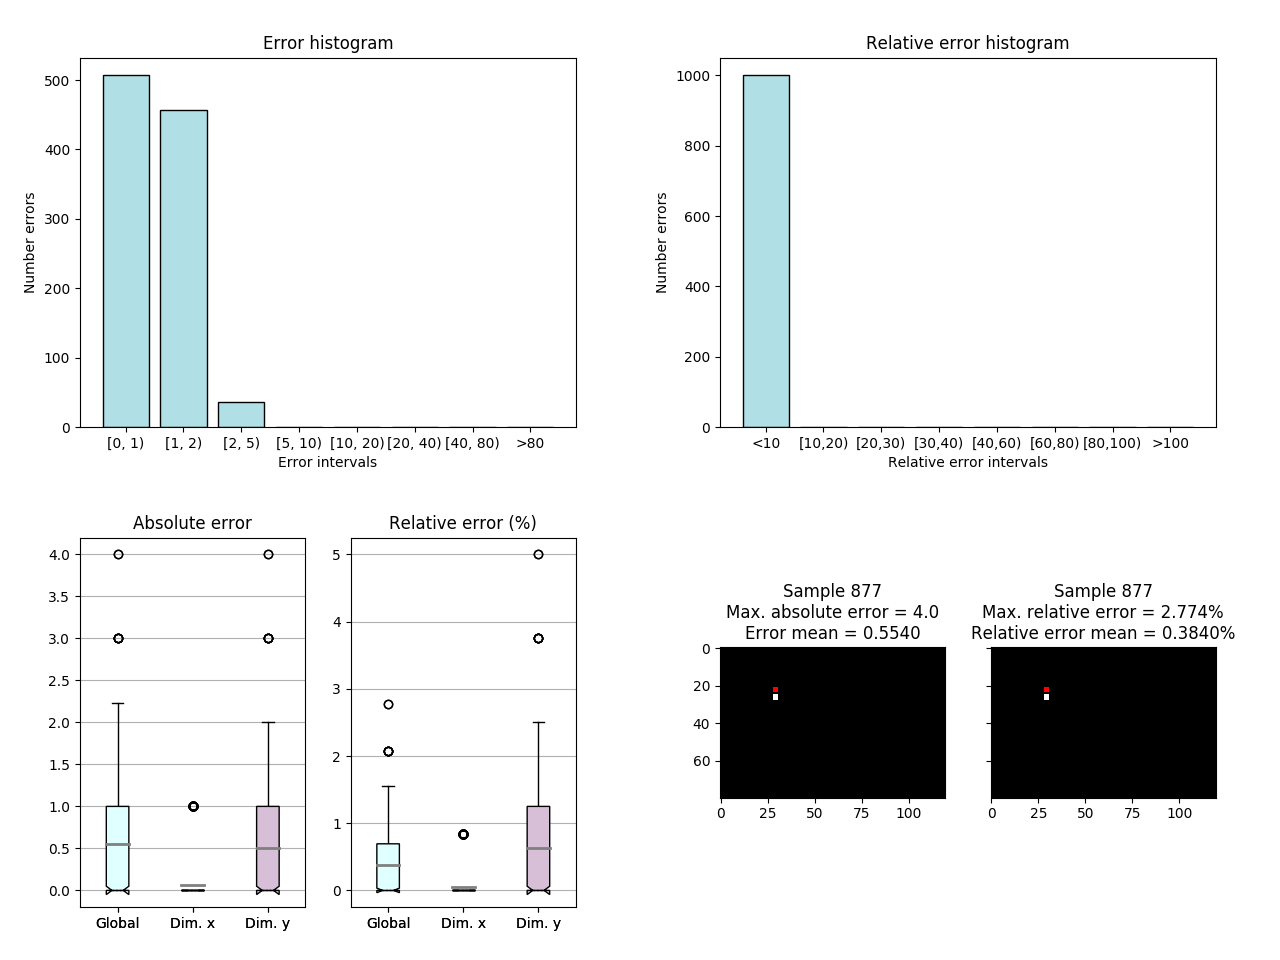
\includegraphics[width=0.8\textwidth]{ figures/test_mod/NOREC/parab_var_10000.png}
			\caption{Resultados de \acrshort{mlp} con dinámica parabólica de 2 \acrshort{dof} en imágenes ~(1000 muestras de \textit{test}).}
			\label{fig.norec_parab_var_10000}
		\end{center}
\end{figure}
\vspace{-30pt}
\begin{figure}[H]
		\begin{center}
			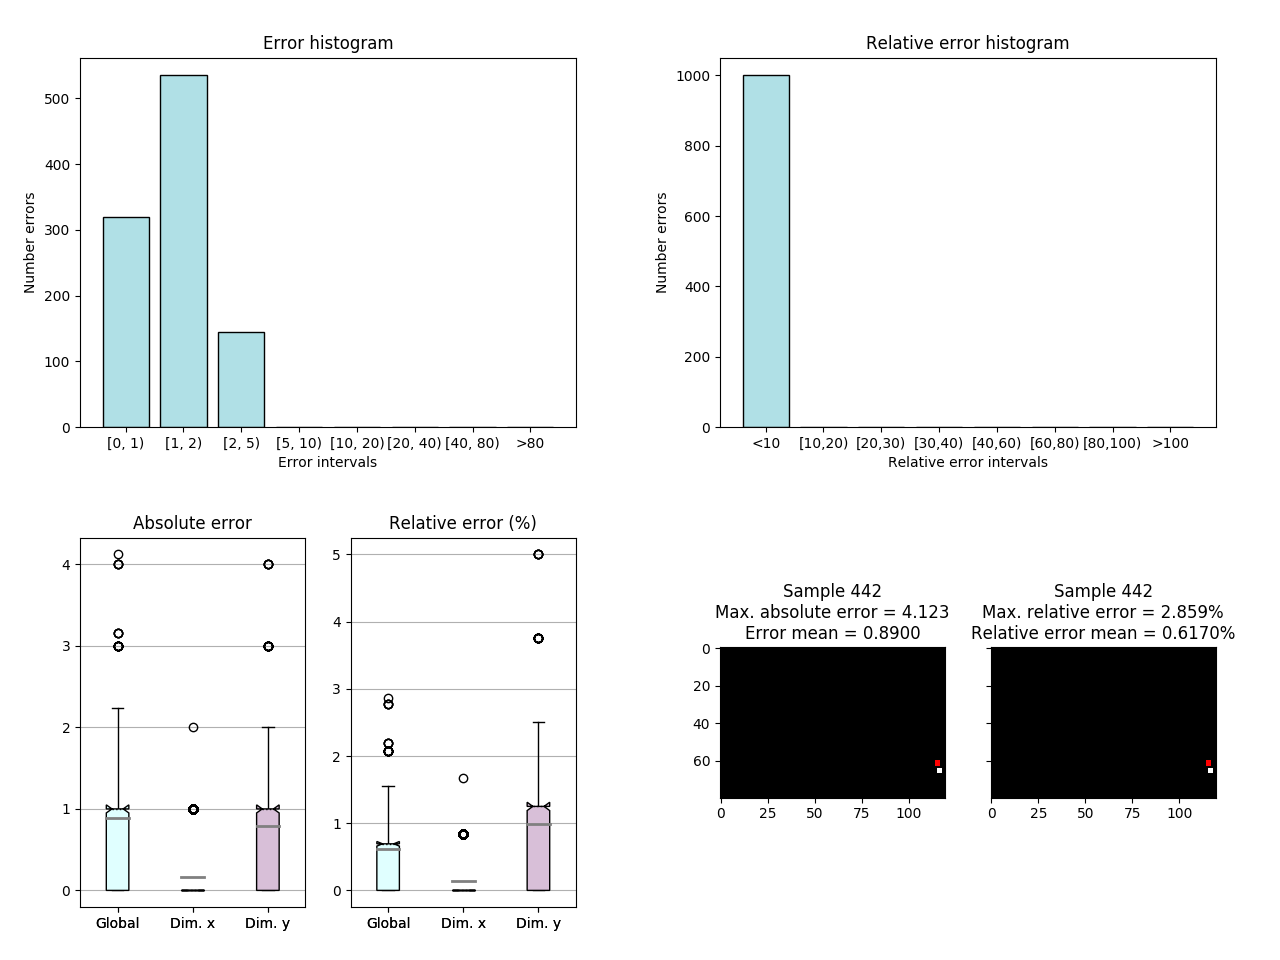
\includegraphics[width=0.8\textwidth]{ figures/test_mod/NOREC/parab_var1_10000.png}
			\caption{Resultados de \acrshort{mlp} con dinámica parabólica de 3 \acrshort{dof}~(1000 muestras de \textit{test}).}
			\label{fig.norec_parab_var1_10000}
		\end{center}
\end{figure}

\subsection{Predicción con dinámicas sinusoidales}
Para abordar la predicción de fotogramas que representan objetos siguen una dinámica sinusoidal se utiliza un \textit{dataset} compuesto por 10000 muestras, dividido de la misma forma que en dinámicas anteriores. En la Figura~\ref{fig.norec_sin_fix_10000} se muestra la evaluación de la estructura de red propuesta cuando el movimiento del píxel sigue una función sinusoidal con un solo \acrshort{dof}, la frecuencia.

\begin{figure}[H]
		\begin{center}
			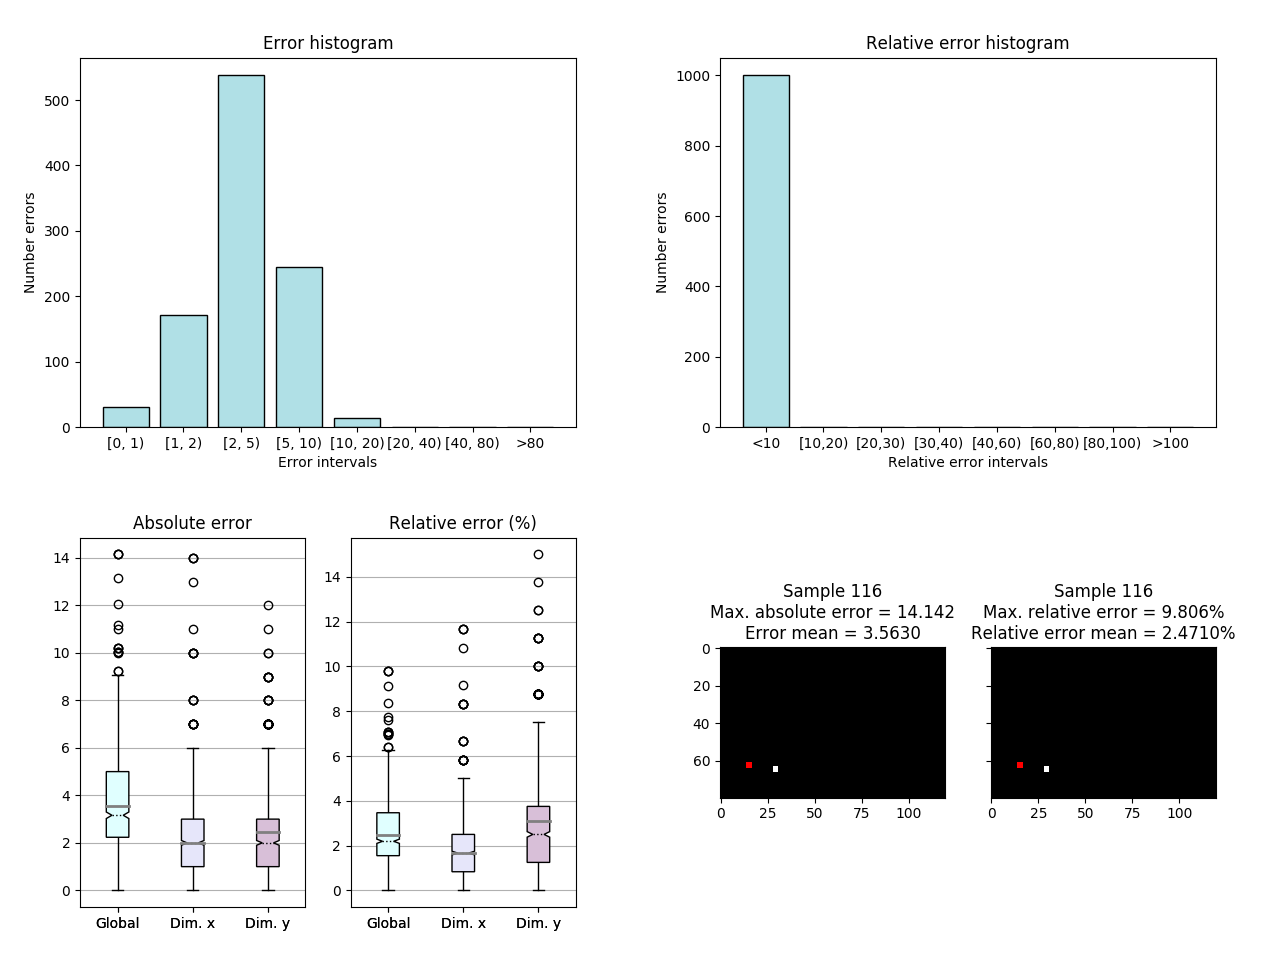
\includegraphics[width=0.8\textwidth]{ figures/test_mod/NOREC/sin_fix_10000.png}
			\caption{Resultados de \acrshort{mlp} con dinámica sinusoidal de 1 \acrshort{dof}~(1000 muestras de \textit{test})).} 
			\label{fig.norec_sin_fix_10000}
		\end{center}
\end{figure}
\vspace{-10pt}

En este caso, los resultados no son tan buenos como los obtenidos para las dinámicas anteriores, que eran más sencillas. Siguiendo la conclusión extraída del Apartado~\ref{ap.muestras}, la solución más inmediata a este deterioro es el aumento de muestras, pasando a un conjunto con un total del 100000 ejemplos: 80000 de entrenamiento, 10000 de validación y 10000 de \textit{test}. Los resultados obtenidos con este nuevo conjunto queda reflejado en los gráficos de la Figura~\ref{fig.norec_sin_fix_100000}.

\begin{figure}[H]
		\begin{center}
			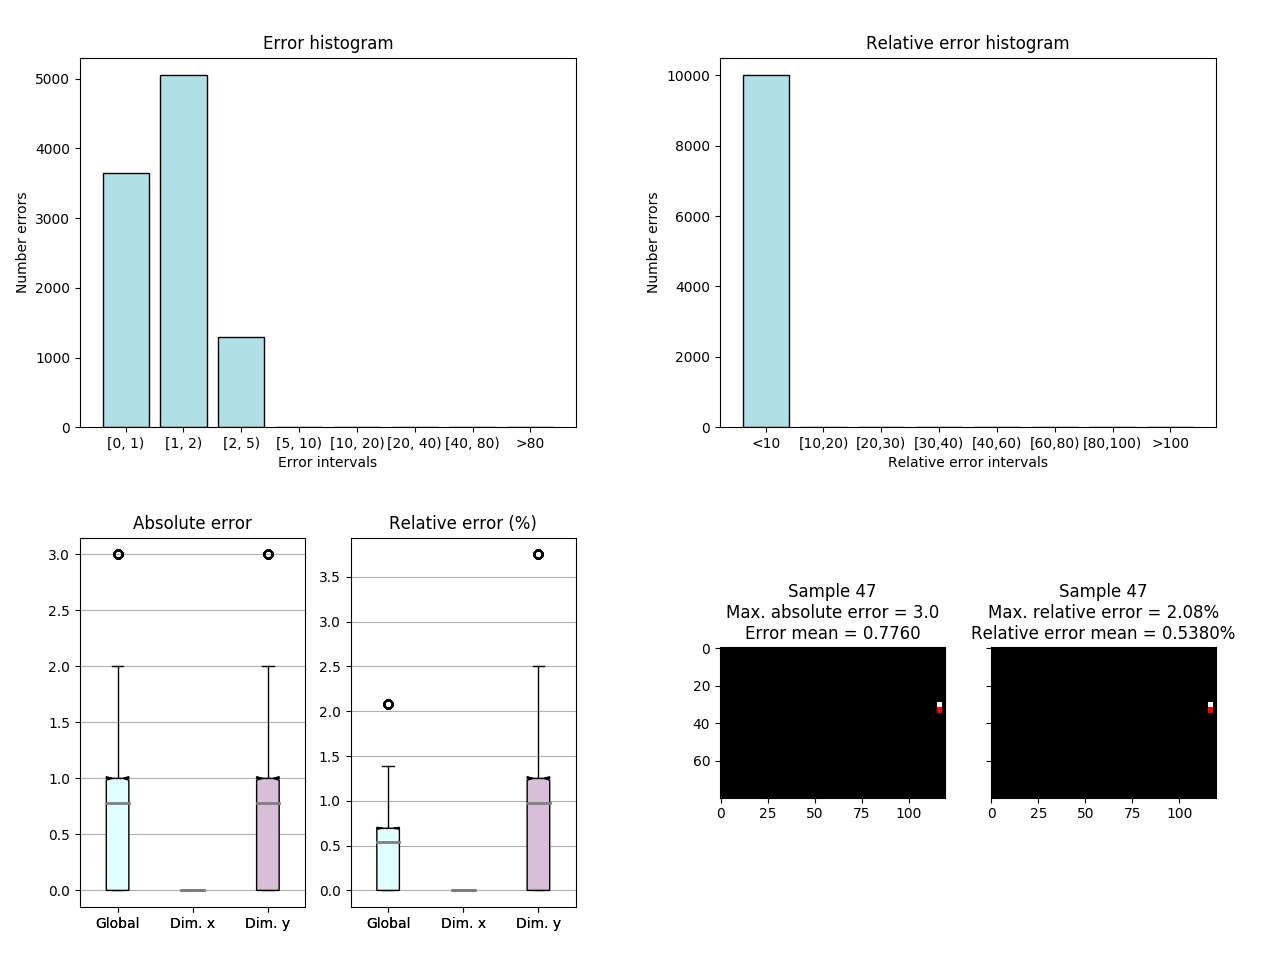
\includegraphics[width=0.8\textwidth]{ figures/test_mod/NOREC/sin_fix_100000.png}
			\caption{Resultados de \acrshort{mlp} con dinámica sinusoidal de 1 \acrshort{dof}~(10000 muestras de \textit{test}).}
			\label{fig.norec_sin_fix_100000}
		\end{center}
\end{figure}
\vspace{-10pt}

Con el incremento en el número de muestras se obtienen mejores resultados en la evaluación, alcanzando la capacidad predictiva conseguida en las dinámicas anteriores.\\

Manteniendo en 100000 el número de muestras, se aumenta la libertad de movimiento del píxel a 2 \acrshort{dof}, con la altura inicial. La red se entrena y evalúa bajo estas premisas dando lugar a los resultados mostrados en la Figura~\ref{fig.norec_sin_var_100000}. Estos datos hacen ver que el aumento de un grado de libertad en esta dinámica incrementa de forma significativa su complejidad, perdiendo la red la capacidad predictiva alcanzada.

\begin{figure}[H]
		\begin{center}
			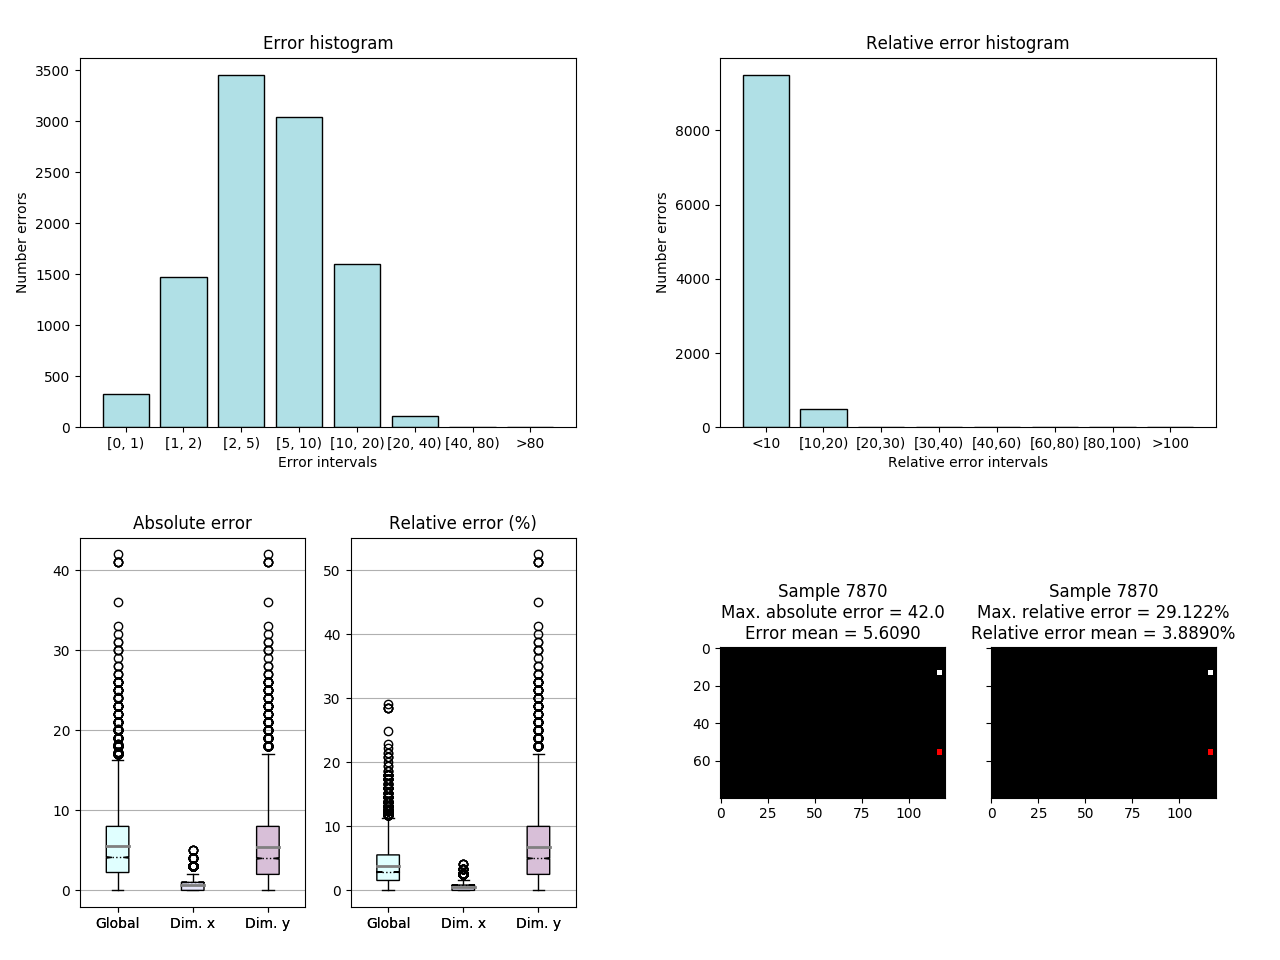
\includegraphics[width=0.8\textwidth]{ figures/test_mod/NOREC/sin_var_100000.png}
			\caption{Resultados de \acrshort{mlp} con dinámica sinusoidal de 2 \acrshort{dof}~(10000 muestras de \textit{test}).}
			\label{fig.norec_sin_var_100000}
		\end{center}
\end{figure}
\vspace{-10pt}

Con estos resultados se concluye que la estructura del \acrshort{mlp} propuesto no es capaz de abarcar la dinámica sinusoidal en su totalidad, poniendo su límite en un único \acrshort{dof}.

\subsection{Resumen de resultados} \label{ap.resumen_RNNmlp}
En la Tabla~\ref{tab.mlp} se muestra un resumen de los resultados alcanzados en cada dinámica.

\begin{table}[H]
	\centering
	\begin{tabular}{{|l|c|c|}}
		\hline
		\multicolumn{2}{|c|}{\textbf{Dinámica}} & \textbf{\acrshort{mlp}}\\ \hline 
		\multirow{2}{*}{Lineal}
		&1~\acrshort{dof} & \cellcolor{darkgreen}{0.21\%}\\
		\cline{2-3}
        &2~\acrshort{dof} & \cellcolor{darkgreen}{0.31\%}\\
        \hline
        \multirow{3}{*}{Parabólica}
        &1~\acrshort{dof} & \cellcolor{darkgreen}0.28\%\\
        \cline{2-3}
        &2~\acrshort{dof} & \cellcolor{darkgreen}0.42\%\\
        \cline{2-3}
        &3~\acrshort{dof} & \cellcolor{darkgreen}0.65\%\\ 
        \hline
        \multirow{2}{*}{Sinusoidal}
        &1~\acrshort{dof} & \cellcolor{darkgreen}0.54\%\\
        \cline{2-3}
        &2~\acrshort{dof} & \cellcolor{myorange}3.89\%\\
        \hline
	\end{tabular}
	\caption{Promedio del error relativo en \textit{test} al evaluar el \acrshort{mlp} con imágenes modeladas y distintas dinámicas (10000 muestras de \textit{test}).}
	\label{tab.mlp}
\end{table}

Para la interpretación de esta tabla se ha establecido un código de cuatro colores que indiquen a simple vista los mejores resultados, en términos de promedio y máximo de error relativo, para cada uno de los casos:

\begin{itemize}
    \item \textbf{Verde oscuro:} Indica muy buenos resultados.
    \item \textbf{Verde claro:} Indica resultados satisfactorios con cierto grado de mejoría.
    \item \textbf{Naranja:} Indica resultados intermedio, generalmente con un buen valor promedio pero un máximo elevado.
    \item \textbf{Rojo:} Indica malos resultados.
\end{itemize}

Además, en el interior de cada celda se refleja el promedio del error relativo de cada uno de los casos para una ilustración cuantitativa de los resultados. Con el objetivo de obtener una evaluación equitativa se han evaluado todas las redes con un conjunto de 10000 muestras, repitiendo la evaluación en aquellas que se utilizaron 1000.
\section{Arquitectura recurrente: LSTM-1}
Otro punto de estudio en el trabajo es el análisis de la capacidad de predicción con redes recurrentes, capaces de captar la relación temporal. Más concretamente se ha optado por el uso de las \acrshort{lstm}, explicadas en el Apartado~\ref{ap.lstm}, por su uso extendido en problemas de esta tipología. En la Figura~\ref{fig.rec_simple_mod} se muestra la estructura de red creada para el caso más sencillo, en el que se emplea una única capa \acrshort{lstm} de 25 neuronas.
\vspace{10pt}
\begin{figure}[H]
		\begin{center}
			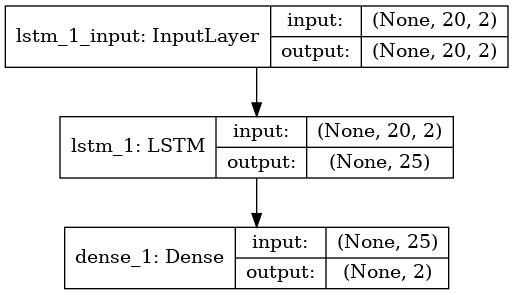
\includegraphics[width=0.6\textwidth]{ figures/net/REC_simple_mod.png}
			\caption{Estructura de LSTM-1 para imágenes modeladas.}
			\label{fig.rec_simple_mod}
		\end{center}
\end{figure}
\vspace{-10pt}

Las entradas y la salida de esta nueva estructura de red coinciden con las establecidas para el \acrshort{mlp}: 20 posiciones como entrada y 1 como salida.

\subsection{Predicción con dinámicas lineales}
Al aplicar la red recurrente sobre los \textit{dataset} cuyo movimiento del píxel en la imagen se rige por la función lineal se obtienen unos resultados muy similares que en el caso no recurrente. En las Figuras~\ref{fig.rec_lin_fix_10000}~y~\ref{fig.rec_lin_var_10000} se puede comprobar cómo se obtienen resultados muy similares a los del \acrshort{mlp}, mejorando ligeramente los resultados en términos de media.\\

\begin{figure}[H]
		\begin{center}
			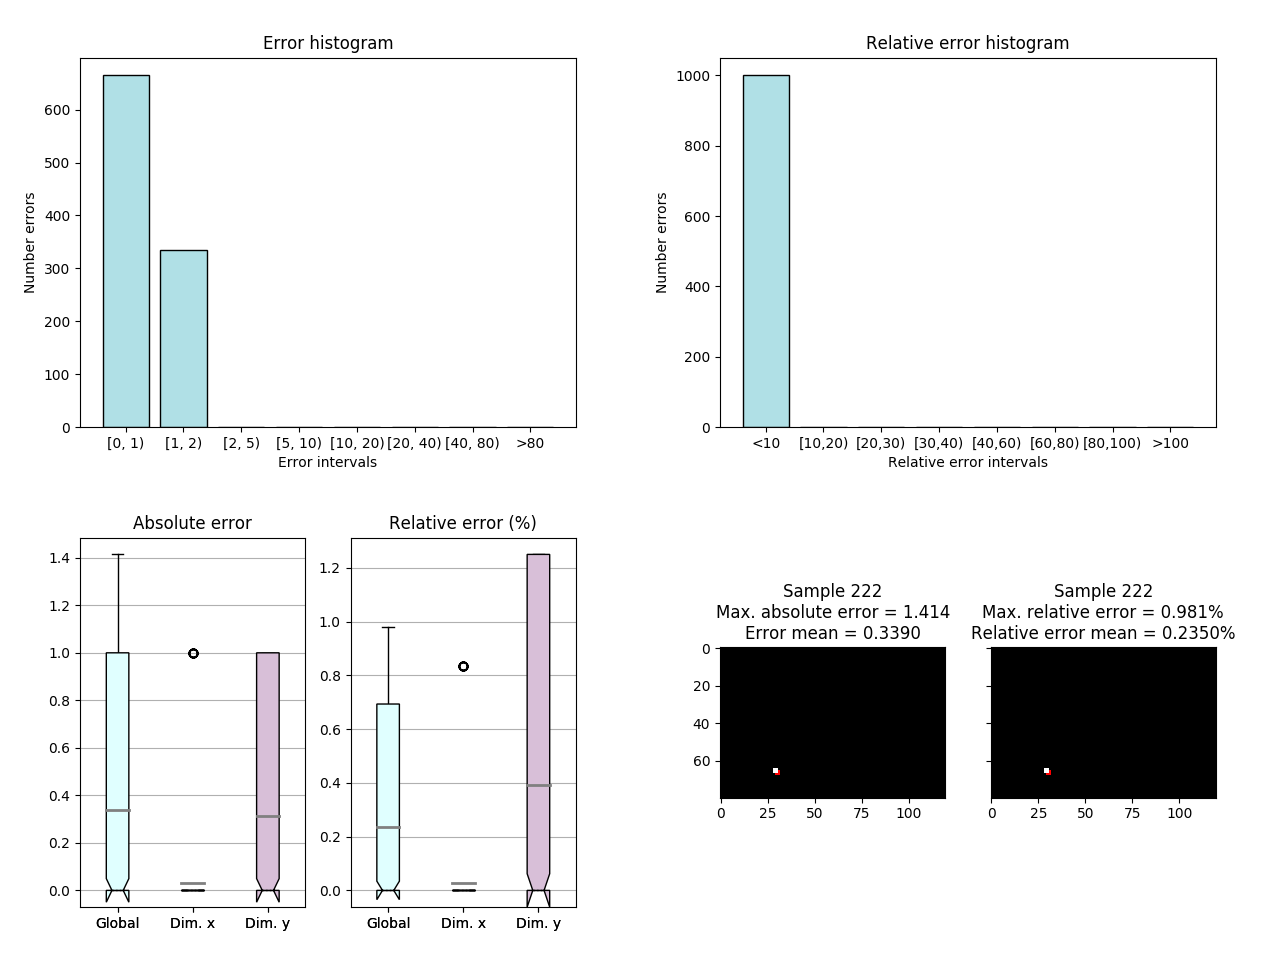
\includegraphics[width=0.8\textwidth]{ figures/test_mod/REC/simple/linear_fix_10000.png}
			\caption{Resultados de LSTM-1 con dinámica lineal de 1 \acrshort{dof}~(1000 muestras de \textit{test}).} 
			\label{fig.rec_lin_fix_10000}
		\end{center}
\end{figure}

\begin{figure}[H]
		\begin{center}
			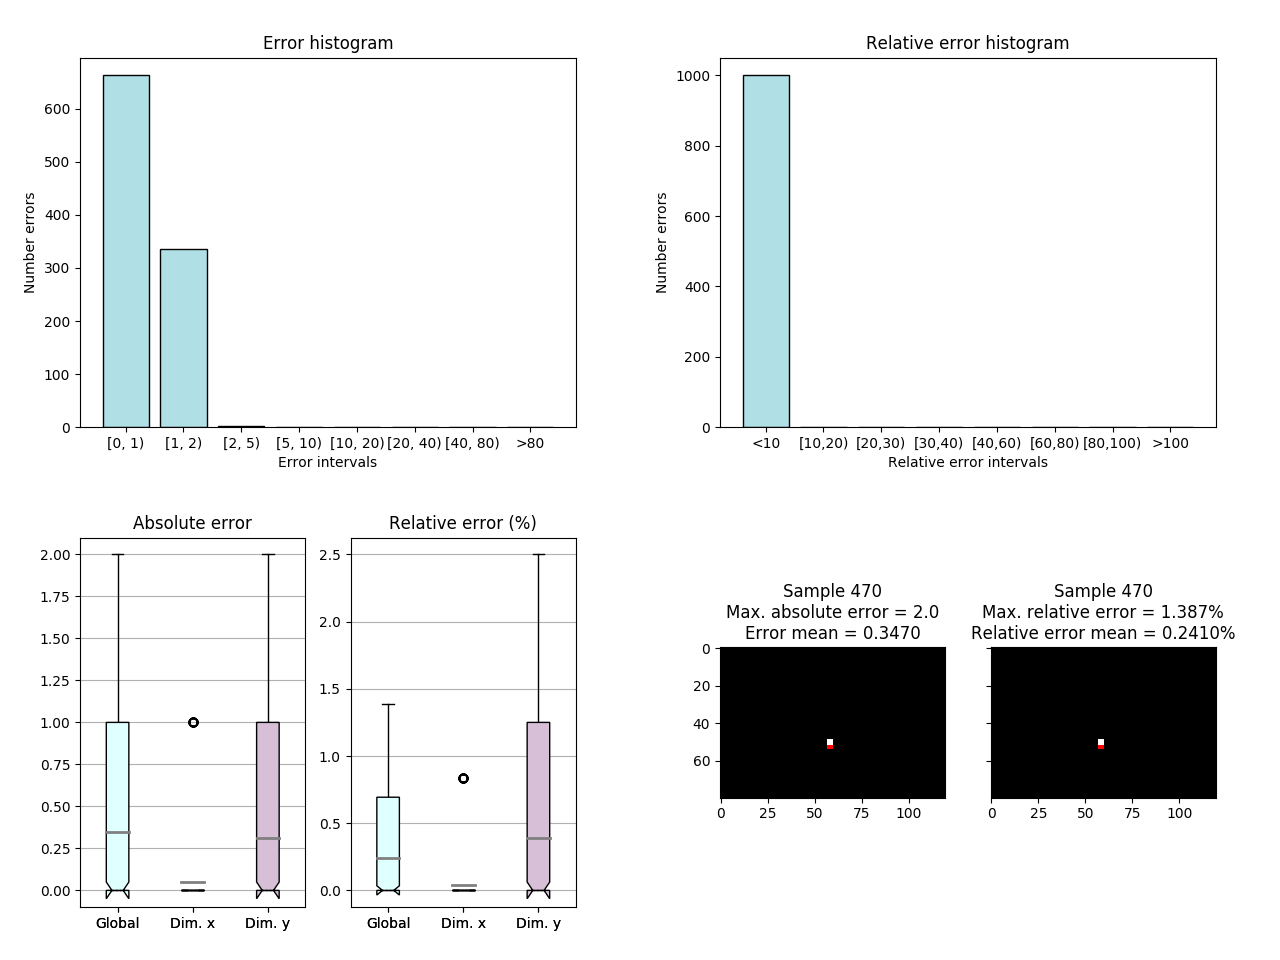
\includegraphics[width=0.8\textwidth]{ figures/test_mod/REC/simple/linear_var_10000.png}
			\caption{Resultados de LSTM-1 con dinámica lineal de 2 \acrshort{dof}~(1000 muestras de \textit{test}).}
			\label{fig.rec_lin_var_10000}
		\end{center}
\end{figure}
\vspace{-10pt}

Estos resultados permiten concluir que en las dinámicas cuyos resultados en el \acrshort{mlp} son buenos, al utilizar redes \acrshort{lstm} la capacidad predictiva se mantiene. Es decir, las redes recurrentes no empeoran significativamente la predicción cuándo ésta funciona sin recurrencia.

\subsection{Predicción con dinámicas parabólicas}
El caso parabólico es muy similar al lineal. Con la red no recurrente ya se consigue que la capacidad predictiva sea buena, por lo que introducir la recurrencia no aportará gran diferencia aunque puede mejorar los resultados. En la Tabla~\ref{tab.mlp_lstm_parab} se muestra una comparación de los resultados obtenidos para esta dinámica con sus 3~\acrshort{dof} y 10000 muestras, tanto con la estructura \acrshort{mlp} como con la \acrshort{lstm}.\\

Estos resultados corroboran lo concluido en el caso lineal: introducir la recurrencia en los casos donde se obtenían buenos resultados, no modifica significativamente los mismos.

\begin{table}[H]
	\centering
	\begin{tabular}{{l|c|c|c|c|}}
		\cline{2-5}
		& \multicolumn{2}{|c|}{\textbf{\acrshort{mlp}}} & \multicolumn{2}{|c|}{\textbf{LSTM-1}} \\
		\hline
		\multicolumn{1}{|l|}{\textbf{\acrshort{dof}}} & \textbf{\textit{Max.}} & \textbf{\textit{Mean}} & \textbf{\textit{Max.}} & \textbf{\textit{Mean}}\\
		\hline 
		\multicolumn{1}{|l|}{\textbf{1~(\textit{a})}} & 1.4\% & 0.2\% & 1.4\% & 0.1\%\\ \hline
		\multicolumn{1}{|l|}{\textbf{2~(\textit{c})}} & 2.8\% & 0.4\% & 2.2\% & 0.3\%\\ \hline
		\multicolumn{1}{|l|}{\textbf{3~(\textit{b})}} & 2.9\% & 0.6\% & 2.3\% & 0.6\%\\ \hline
	\end{tabular}
	\caption{Error relativo en la dinámica parabólica con \acrshort{mlp} y LSTM-1 (1000 muestras de \textit{test})).}
	\label{tab.mlp_lstm_parab}
\end{table}

\subsection{Predicción con dinámicas sinusoidales}
En la dinámica sinusoidal, con el \acrshort{mlp}, únicamente se conseguía dominar el caso más sencillo de 1 \acrshort{dof} (frecuencia). En la Figura~\ref{fig.rec_sin_fix_100000} se muestran los resultados obtenidos para este caso utilizando la estructura recurrente propuesta. Se mantienen los buenos resultados arrojados por el \acrshort{mlp}, reforzando las conclusiones extraídas.\\

\begin{figure}[H]
		\begin{center}
			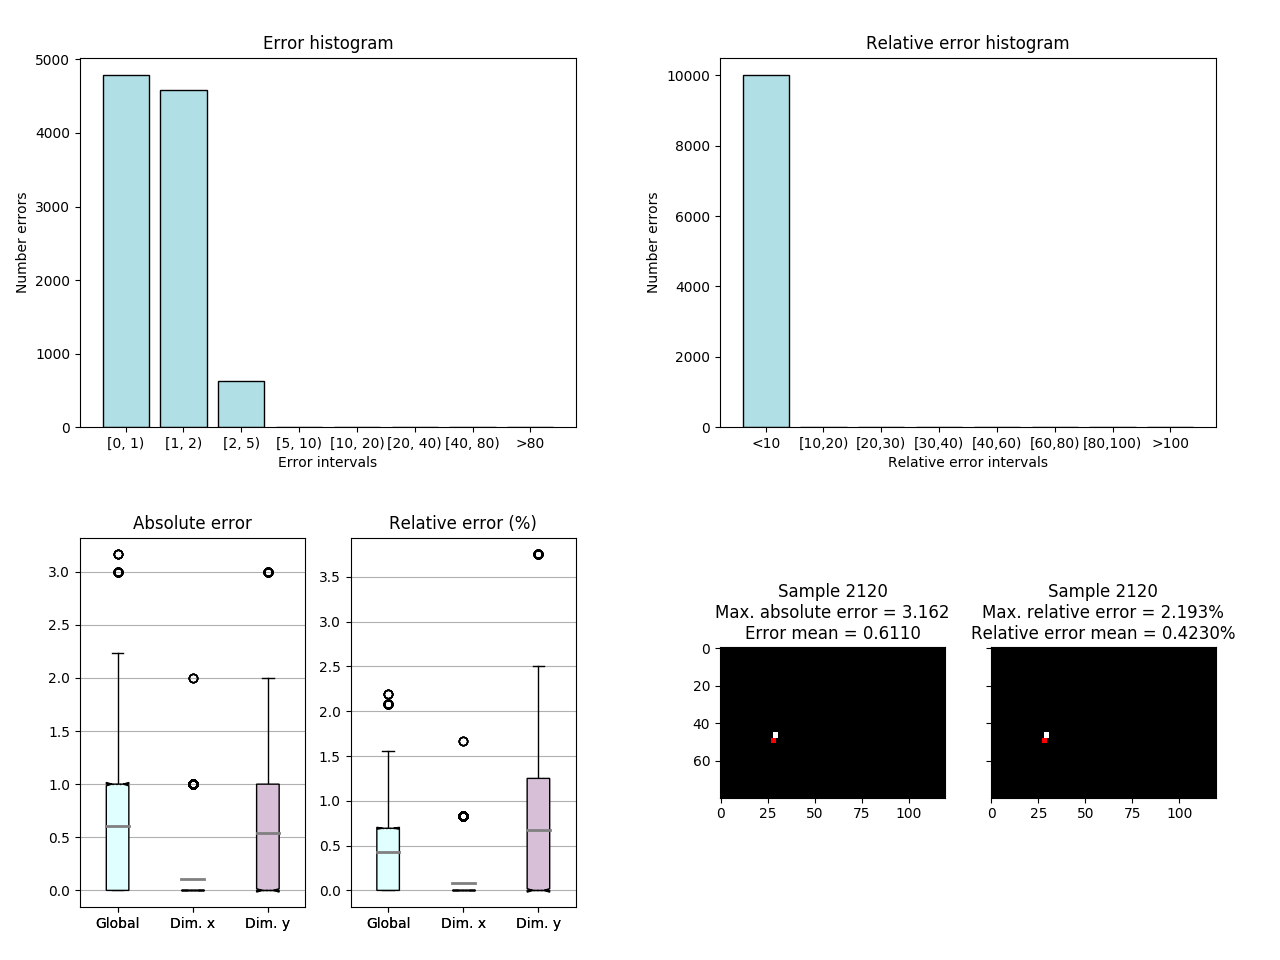
\includegraphics[width=0.8\textwidth]{ figures/test_mod/REC/simple/sin_fix_100000.png}
			\caption{Resultados de LSTM-1 con dinámica sinusoidal de 1 \acrshort{dof}~(10000 muestras de \textit{test}).}
			\label{fig.rec_sin_fix_100000}
		\end{center}
\end{figure}

Al complicar la dinámica con el aumento de la libertad de movimiento del píxel, la red no recurrente estudiada no es capaz de predecir correctamente. Se espera que al introducir la recurrencia, no solo se mantengan los resultados como anteriormente, sino que la capacidad predictiva en estos casos mejore considerablemente. En la Figura~\ref{fig.rec_sin_var_100000} se muestran los resultados del primer experimento en este sentido. Se entrena y evalúa la red recurrente propuesta con un conjunto de 100000 muestras y permitiendo 2 \acrshort{dof}, frecuencia y altura inicial.

\begin{figure}[H]
		\begin{center}
			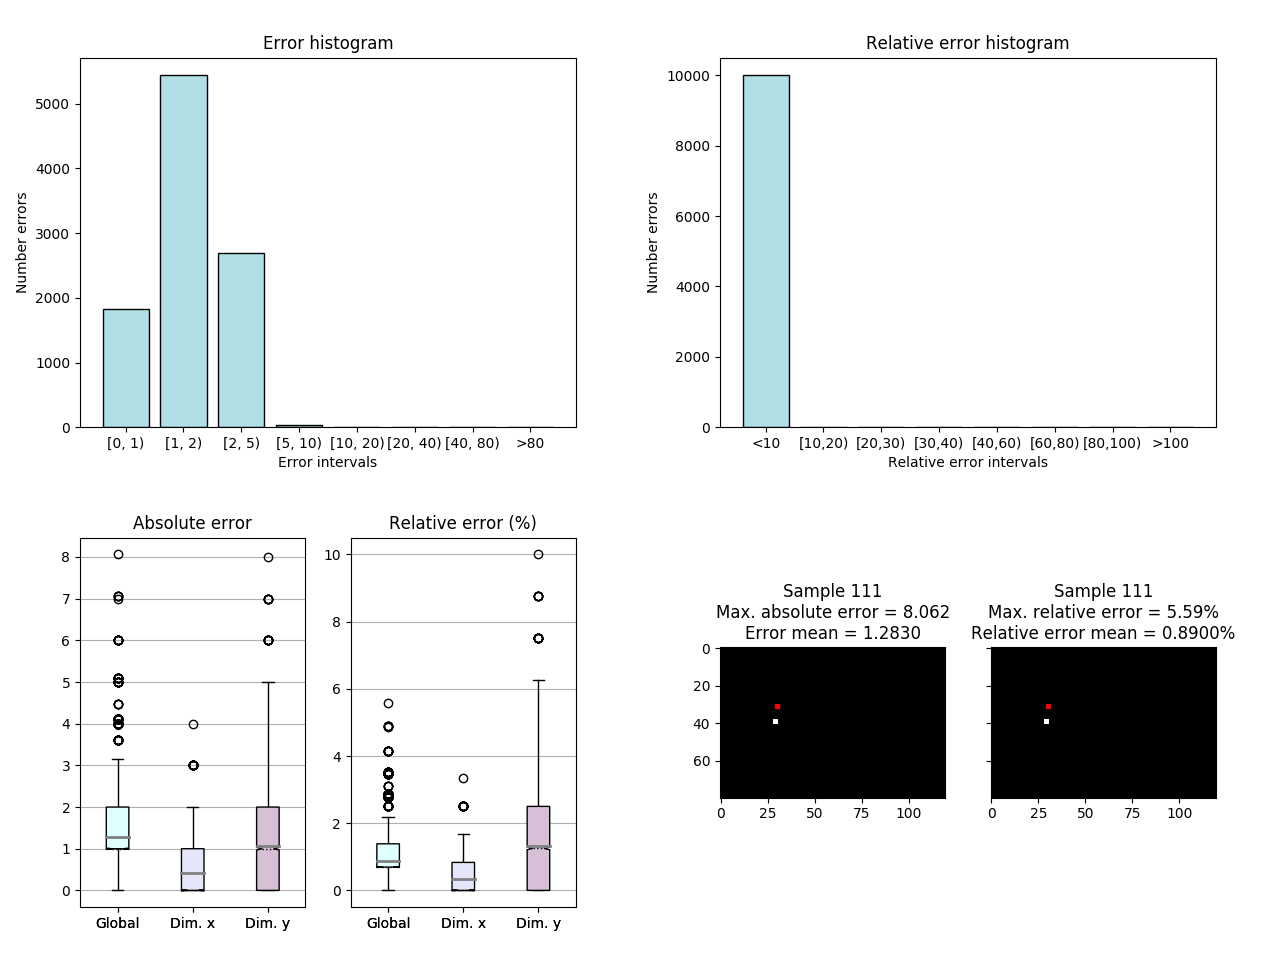
\includegraphics[width=0.8\textwidth]{ figures/test_mod/REC/simple/sin_var_100000.png}
			\caption{Resultados de LSTM-1 con dinámica sinusoidal de 2 \acrshort{dof}~(10000 muestras de \textit{test}).}
			\label{fig.rec_sin_var_100000}
		\end{center}
\end{figure}
\vspace{-10pt}

Se puede observar una mejora considerable respecto a los resultados de la Figura~\ref{fig.norec_sin_var_100000}, que evalúa una red no recurrente bajo las mismas circunstancias. Esta comparación corrobora la idea mencionada anteriormente de que la recurrencia mejora la capacidad predictiva de una red cuando esta no es es del todo buena.\\

Se añade un nuevo \acrshort{dof} a la dinámica, la amplitud y se realiza el entrenamiento y evaluación con un conjunto del mismo número de muestras~(100000) que en los casos anteriores. En la Figura~\ref{fig.rec_sin_var1_100000} se muestran los resultados para este caso.

\begin{figure}[H]
		\begin{center}
			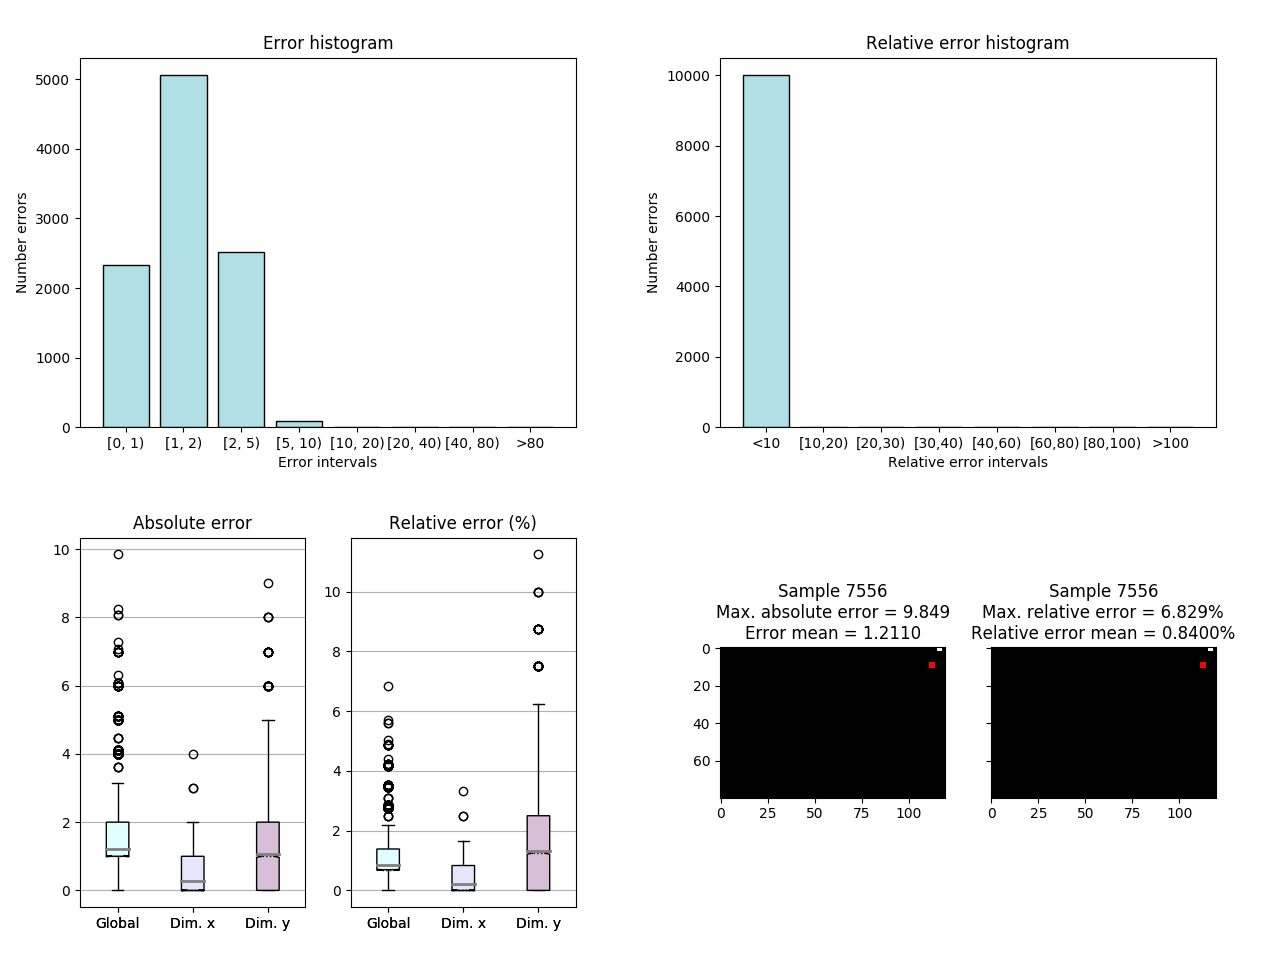
\includegraphics[width=0.8\textwidth]{ figures/test_mod/REC/simple/sin_var1_100000.png}
			\caption{Resultados de LSTM-1 con dinámica sinusoidal de 3 \acrshort{dof}~(10000 muestras de \textit{test}).}
			\label{fig.rec_sin_var1_100000}
		\end{center}
\end{figure}
\vspace{-10pt}

Los resultados obtenidos indican que la red tiene una buena capacidad predictiva, lo que refuerza la idea de que introducir la recurrencia en problemas de esta naturaleza facilita la tarea de predicción.\\

Se entrena la red con el siguiente grado de complejidad, 4~\acrshort{dof}, cuyos resultados se reflejan en la Figura~\ref{fig.rec_sin_var2_100000}. Para este último caso, el más complejo de la dinámica, la red no tiene una buena capacidad predictiva a pesar de introducir la recurrencia. Este hecho puede derivarse de la sencillez de la propia red propuesta, que dispone de una única capa con 25 neuronas, algo que se tratará posteriormente.

\begin{figure}[H]
		\begin{center}
			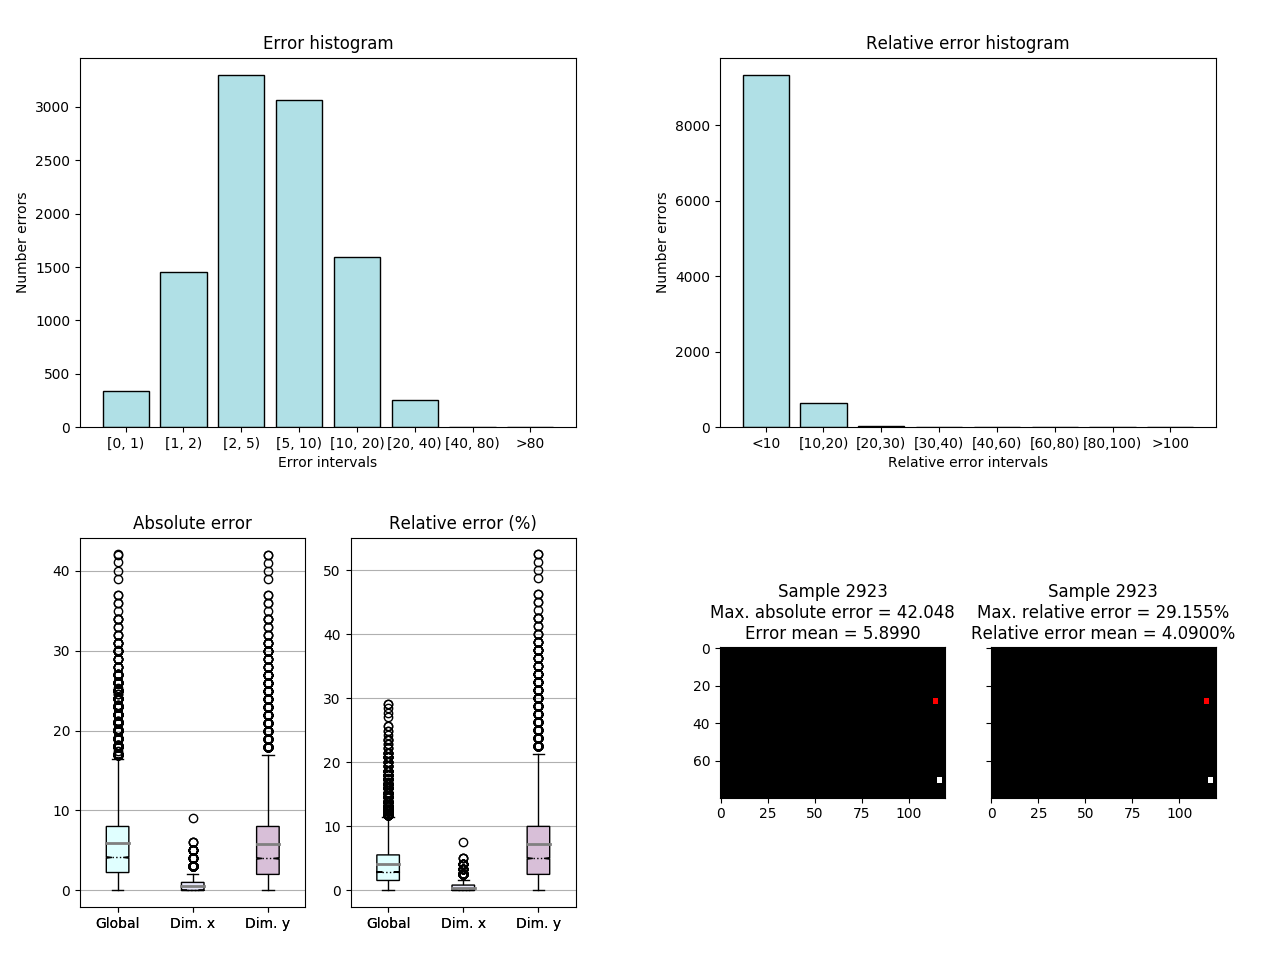
\includegraphics[width=0.8\textwidth]{ figures/test_mod/REC/simple/sin_var2_100000.png}
			\caption{Resultados de LSTM-1 con dinámica sinusoidal de 4 \acrshort{dof}~(10000 muestras de \textit{test}).}
			\label{fig.rec_sin_var2_100000}
		\end{center}
\end{figure}
\vspace{-20pt}
\subsection{Resumen de resultados}
La Tabla~\ref{tab.lstm1} resume los resultados obtenidos con la red \textit{LSTM-1} para cada dinámica.

\begin{table}[H]
	\centering
	\begin{tabular}{{|l|c|c|}}
		\hline
		\multicolumn{2}{|c|}{\textbf{Dinámica}} & \textbf{LSTM-1}\\ \hline 
		\multirow{2}{*}{Lineal}
		&1~\acrshort{dof} & \cellcolor{darkgreen}0.16\%\\
		\cline{2-3}
        &2~\acrshort{dof} & \cellcolor{darkgreen}0.25\%\\ 
        \hline
        \multirow{3}{*}{Parabólica}
        &1~\acrshort{dof} & \cellcolor{darkgreen}0.12\%\\
        \cline{2-3}
        &2~\acrshort{dof} & \cellcolor{darkgreen}0.35\%\\
        \cline{2-3}
        &3~\acrshort{dof} & \cellcolor{darkgreen}0.58\%\\ 
        \hline
        \multirow{4}{*}{Sinusoidal}
        &1~\acrshort{dof} & \cellcolor{darkgreen}0.42\%\\
        \cline{2-3}
        &2~\acrshort{dof} & \cellcolor{greenyellow}0.89\%\\
        \cline{2-3}
        &3~\acrshort{dof} & \cellcolor{greenyellow}0.84\%\\
        \cline{2-3}
        &4~\acrshort{dof} & \cellcolor{myorange}4.1\%\\ 
        \hline
	\end{tabular}
	\caption{Promedio del error relativo en \textit{test} al evaluar la red LSTM-1 con imágenes modeladas y distintas dinámicas (10000 muestras de \textit{test}).}
	\label{tab.lstm1}
\end{table}

Al igual que en el caso anterior se han evaluado todas las redes con un conjunto de 10000 muestras para una comparación equitativa, repitiendo la evaluación en aquellas que se utilizaron 1000.

\section{Arquitectura recurrente: LSTM-4}
Para tratar de obtener una arquitectura capaz de predecir en todas las dinámicas en su caso más complejo se realizan una serie de experimentos que dan lugar a la estructura recurrente definida en la Figura~\ref{fig.rec_complex_mod}.

\begin{figure}[H]
		\begin{center}
			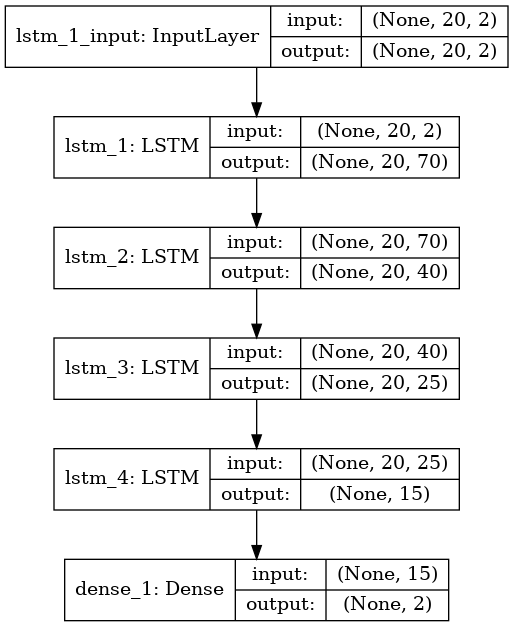
\includegraphics[width=0.67\textwidth]{ figures/net/REC_complex_mod.png}
			\caption{Estructura de LSTM-4 para imágenes modeladas.}
			\label{fig.rec_complex_mod}
		\end{center}
\end{figure}
\vspace{-10pt}
Esta nueva red está compuesta por 4 capas \acrshort{lstm} de 70, 40, 25 y 15 neuronas respectivamente, cuya entrada son las 20 posiciones conocidas y la salida la posición futura estimada.\\
\indent Para llegar a definir la nueva estructura de red se han explorado dos vías: el aumento de neuronas y el de capas, que serán explicados a continuación. Además, se presentan los resultados obtenidos para cada una de las dinámicas consideradas.
\subsection{Aumento de neuronas}
Una vía para la mejora de la red recurrente en las imágenes modeladas es el aumento de neuronas manteniendo una única capa. En este sentido, se duplica el número de neuronas, pasando de las 25 provistas para la red \textit{LSTM-1} a un total de 50. Con esta nueva red, utilizando el conjunto de 100000 muestras que sigue la dinámica sinusoidal con 4~\acrshort{dof}, se obtienen los resultados de la Figura~\ref{fig.units_rec_sin_var2_100000}.

\begin{figure}[H]
		\begin{center}
			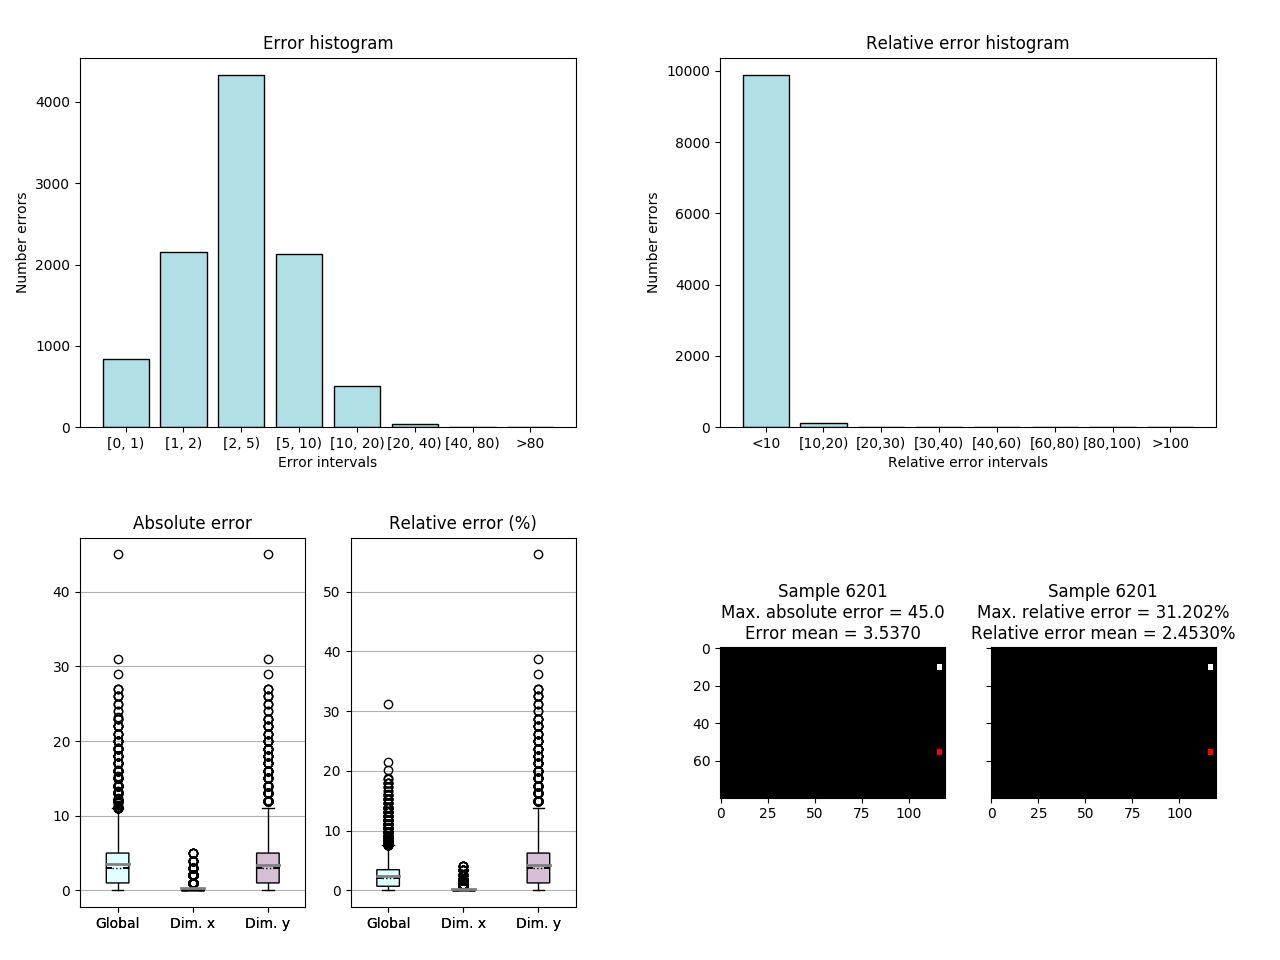
\includegraphics[width=0.8\textwidth]{ figures/test_mod/REC/complex/units_sin_var2_100000.png}
			\caption{Resultados de \acrshort{lstm} de 50 neuronas con dinámica sinusoidal de 4 \acrshort{dof}~(10000 muestras de \textit{test}).}
			\label{fig.units_rec_sin_var2_100000}
		\end{center}
\end{figure}
\vspace{-10pt}

Al comparar los resultados con los equivalentes para la red con menor número de neuronas, en la Figura ~\ref{fig.rec_sin_var2_100000}, se observa una mejora en promedio del error relativo. Este hecho parece corroborar la idea de que la poca capacidad predictiva de la red \textit{LSTM-1}, bajo estas circunstancias, es consecuencia de su simplicidad. Sin embargo, esta mejora no es suficiente para lograr una red que sea capaz de predecir en el caso más complejo.

\subsection{Aumento de capas} \label{ap.capas_mod}
La segunda vía a explorar en la mejora de la red \textit{LSTM-1} es el aumento de del número de capas. En este sentido, se comienza con el aumento de una única capa, que ya proporciona unos datos mucho mejores que los expuestos anteriormente. Este hecho hace ver que esta mecánica es más efectiva que el aumento de neuronas, y reafirma la idea de que una red más compleja captará mejor las distintas relaciones.\\

Con la idea de que el aumento del número de capas es la estrategia más efectiva, se debe establecer el límite de capas a añadir. Para ello se realiza un estudio en el que se aumenta de forma gradual el número de capas, disminuyendo de la misma forma el número de neuronas en cada una de ellas. En la Figura~\ref{fig.capas_mod} se muestra un gráfico en el que se representa la evolución del valor del error relativo, en términos de media y máximo, a medida que se aumentan las capas. Para la elaboración de esta tabla se ha utilizado el mismo conjunto que en el aumento de neuronas, 100000 muestras de sinusoidal con todos sus~\acrshort{dof}.

\begin{figure}[H]
		\begin{center}
			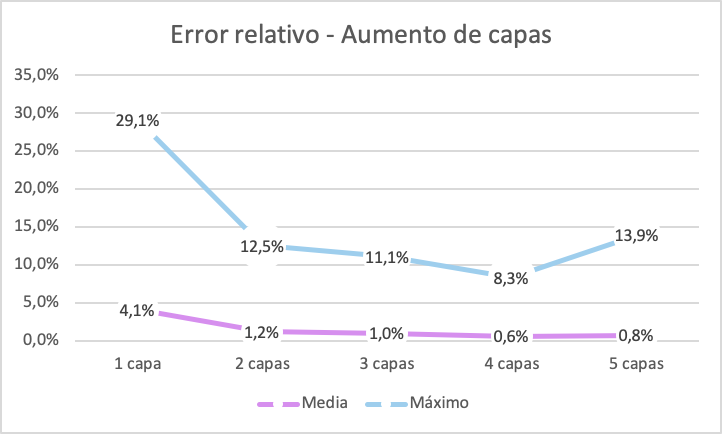
\includegraphics[width=0.7\textwidth]{ figures/test_mod/REC/complex/capas_mod.png}
			\caption{Comparación del error relativo al aumentar el número de capas \acrshort{lstm}~(Sinusoidal, 4~\acrshort{dof}, 10000 muestras de \textit{test}).}
			\label{fig.capas_mod}
		\end{center}
\end{figure}
\vspace{-10pt}

En esta gráfica se puede comprobar que los resultados mejoran a medida que se añaden más capas, hasta llegar a 4 capas. Cuando se emplean 5 capas el error vuelve a subir, empeorando los resultados, lo que hace que se opte por definir la estructura con 4 capas \acrshort{lstm}.

\subsection{Predicción con dinámicas lineales}
En la Figura~\ref{fig.complex_rec_lin_var_100000} se muestran los resultados obtenidos para la dinámica lineal de 2~\acrshort{dof} con esta nueva estructura de red.

\begin{figure}[H]
		\begin{center}
			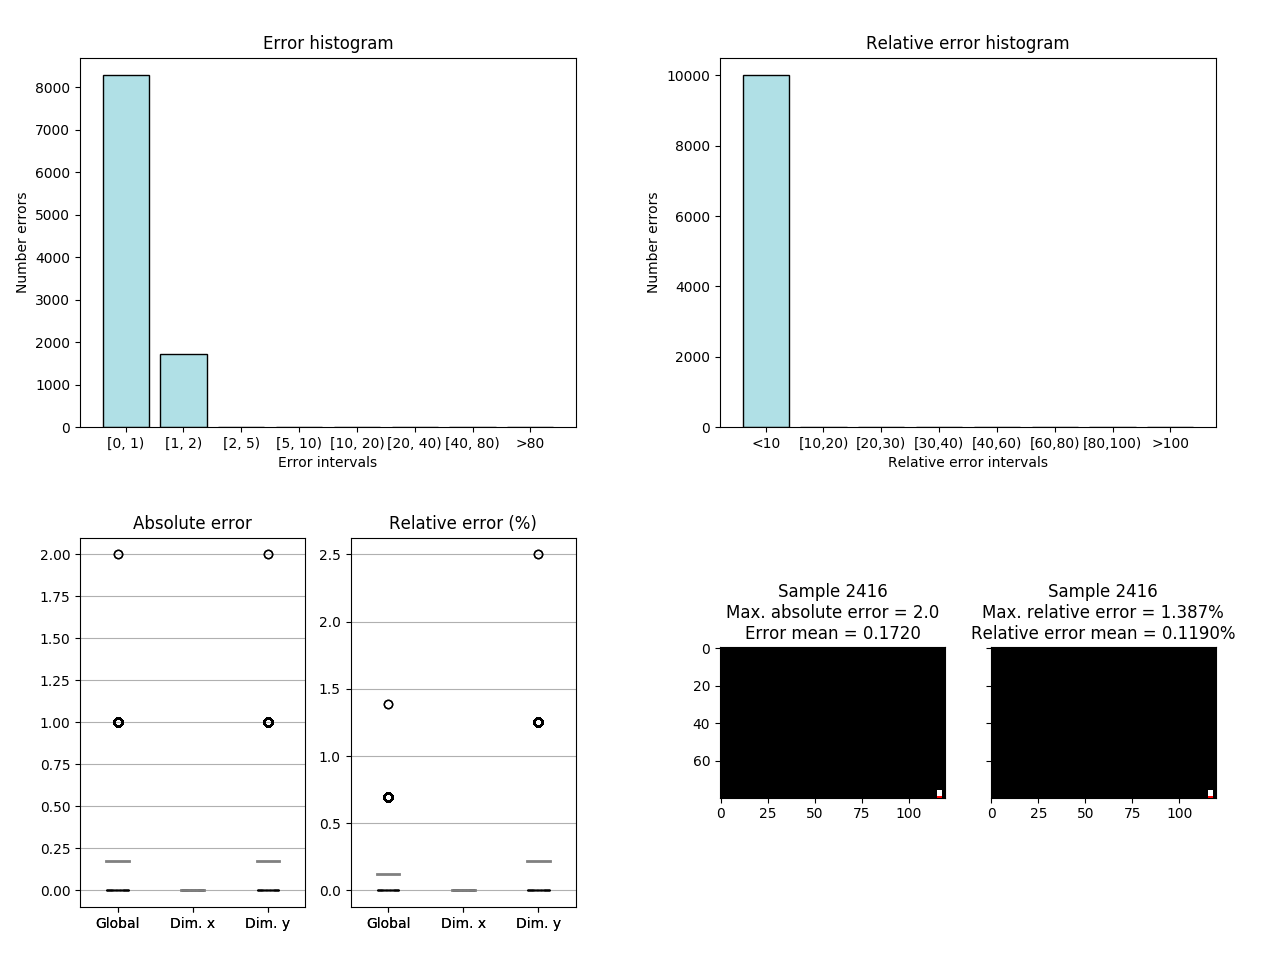
\includegraphics[width=0.8\textwidth]{ figures/test_mod/REC/complex/linear_var_100000.png}
			\caption{Resultados de LSTM-4 con dinámica lineal de 2 \acrshort{dof}~(10000 muestras de \textit{test}).} 
			\label{fig.complex_rec_lin_var_100000}
		\end{center}
\end{figure}
\vspace{-10pt}
Los resultados obtenidos son muy similares a los de la estructura \acrshort{lstm} con una única capa y 10000 muestras. Este hecho hace concluir que, aunque los resultados son muy buenos, no compensa el aumento del coste computacional pues no se obtiene una mejora significativa.

\subsection{Predicción con dinámicas parabólicas}
Para esta dinámica, cuyo máximo grado de complejidad se alcanza al tener 3~\acrshort{dof}, los resultados obtenidos al evaluar la estructura de red propuesta se muestran en la Figura~\ref{fig.complex_rec_parab_var1_100000}.

\begin{figure}[H]
		\begin{center}
			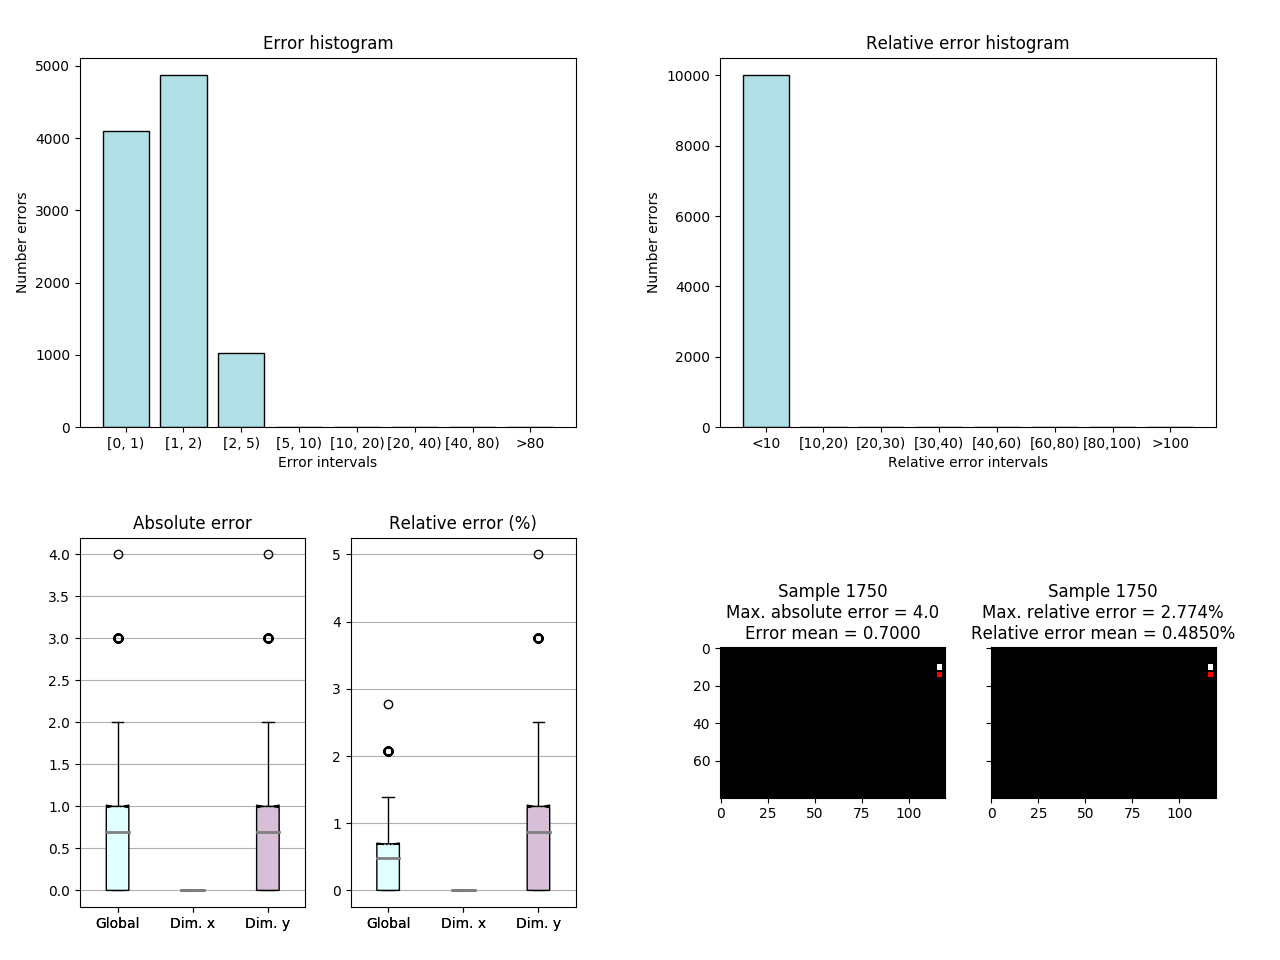
\includegraphics[width=0.8\textwidth]{ figures/test_mod/REC/complex/parab_var1_100000.png}
			\caption{Resultados de LSTM-4 con dinámica parabólica de 3 \acrshort{dof}~(10000 muestras de \textit{test}).} 
			\label{fig.complex_rec_parab_var1_100000}
		\end{center}
\end{figure}
\vspace{-10pt}

Al igual que ocurre en el caso anterior, la capacidad de predicción de la red \textit{LSTM-1} ya es buena para esta dinámica con un conjunto de 10000 muestras. Los resultados arrojados al utilizar un conjunto más grande con una estructura más compleja reafirman lo concluido en el caso lineal: no compensa el coste computacional por la mejora.

\subsection{Predicción con dinámicas sinusoidales}
La última dinámica considerada hasta el momento, regida por la función sinusoidal, establece su máxima complejidad en 4~\acrshort{dof}. Los resultados de entrenar y evaluar la nueva red con el \textit{dataset} de 100000 muestras y dichos grados de libertad se muestran en la Figura~\ref{fig.complex_rec_sin_var2_100000}.

\begin{figure}[H]
		\begin{center}
			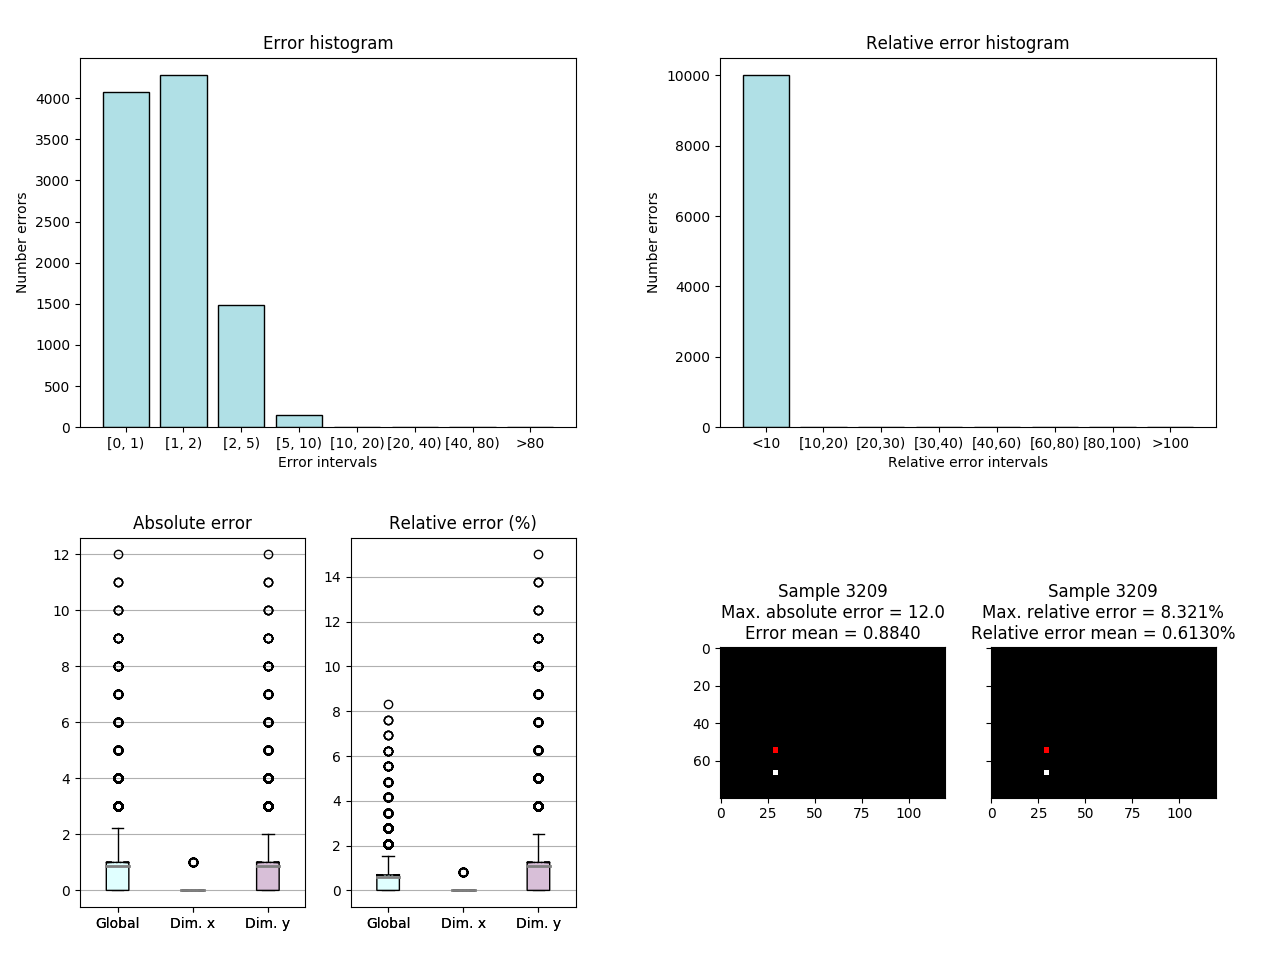
\includegraphics[width=0.8\textwidth]{ figures/test_mod/REC/complex/layers_sin_var2_100000.png}
			\caption{Resultados de LSTM-4 con dinámica sinusoidal de 4 \acrshort{dof}~(10000 muestras de \textit{test}).} 
			\label{fig.complex_rec_sin_var2_100000}
		\end{center}
\end{figure}
\vspace{-10pt}

En esta última dinámica no se habían conseguido unos resultados demasiado buenos con la estructura \textit{LSTM-1}, había un alto grado de incertidumbre. Con la nueva estructura de red los resultados de la misma mejoran considerablemente, lo que hace que se pueda predecir con mayor certeza. Por tanto, sí que resulta efectivo aumentar la complejidad y, con ello el coste computacional, por una mejora en la capacidad predictiva para la dinámica.

\subsection{Predicción con dinámica combinada}
Tras haber dominado por separado las dinámicas en su grado más complejo, se ha considerado un nuevo conjunto que contiene 33000 ejemplos lineales y parabólicos, y 34000 sinusoidales, con el objetivo de explorar una dinámica combinada. La red se entrena y evalúa con este nuevo conjunto y se obtienen los resultados mostrados en la Figura~\ref{fig.complex_rec_mix_100000}.

\begin{figure}[H]
		\begin{center}
			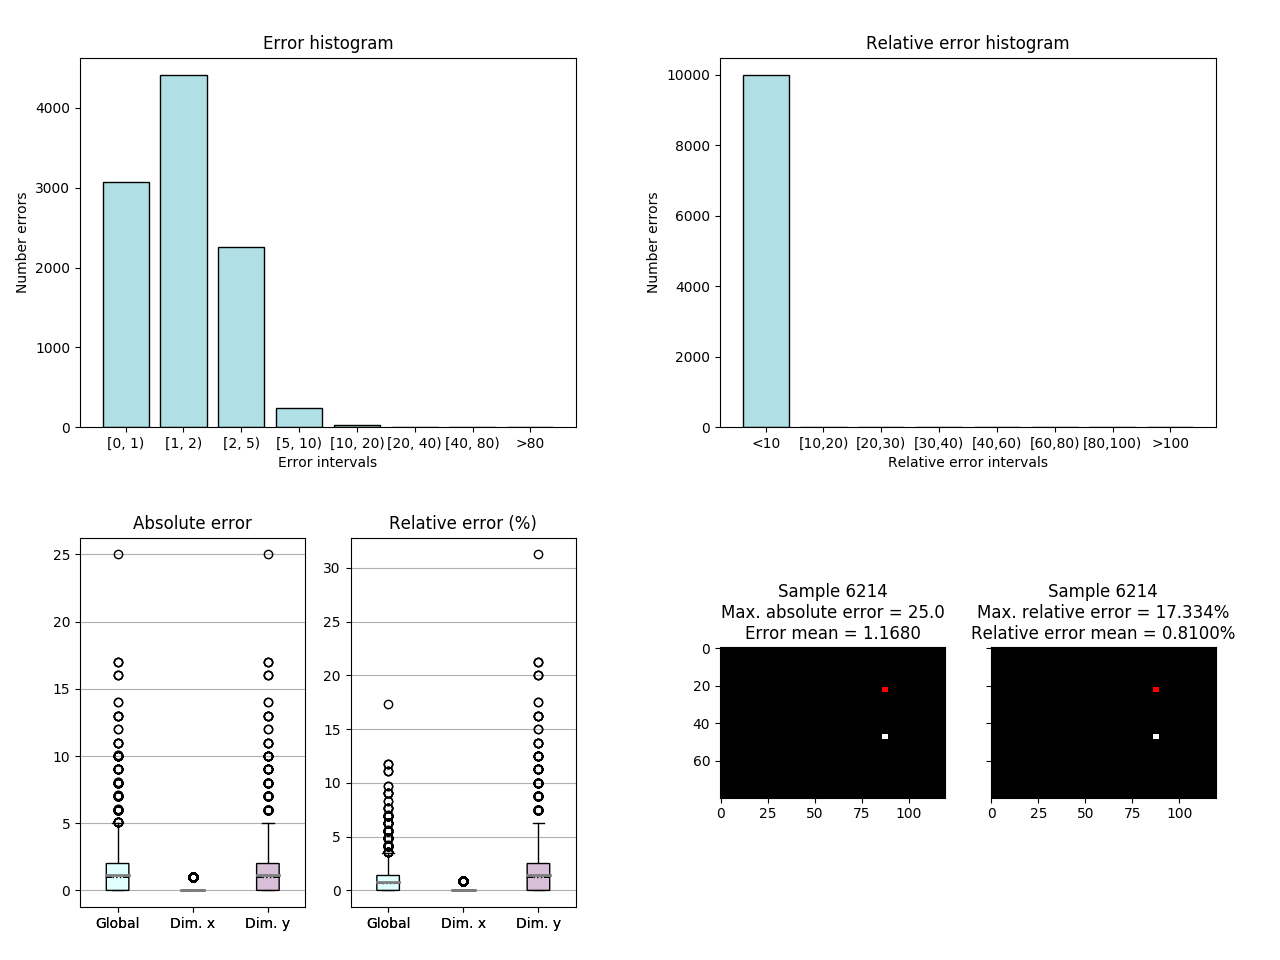
\includegraphics[width=0.8\textwidth]{ figures/test_mod/REC/complex/mix_100000.png}
			\caption{Resultados de LSTM-4 con dinámica combinada~(10000 muestras de \textit{test}).} 
			\label{fig.complex_rec_mix_100000}
		\end{center}
\end{figure}
\vspace{-10pt}

Los resultados están limitados por los obtenidos para cada dinámica por separado. Al mezclar las muestras en la misma proporción, con algún ejemplo más de la sinusoidal, no se espera mejorar los resultados de la que peor predice. De esta forma, aunque se comete mayor error respecto al caso sinusoidal, se consigue mantener la capacidad de predicción en términos generales.

\subsection{Predicción a largo plazo} 
El último experimento propuesto en cuanto a la predicción de las imágenes modeladas consiste en el análisis de la repercusión del horizonte temporal en la calidad de la predicción. Para ello se ha utilizado el conjunto de la dinámica combinada con 100000 muestras incrementando el valor del \textit{gap} gradualmente. En la Figura~\ref{fig.gap} se muestra la evolución del error relativo obtenido, en términos de media y máximo, a medida que se modifica este parámetro.

\begin{figure}[H]
		\begin{center}
			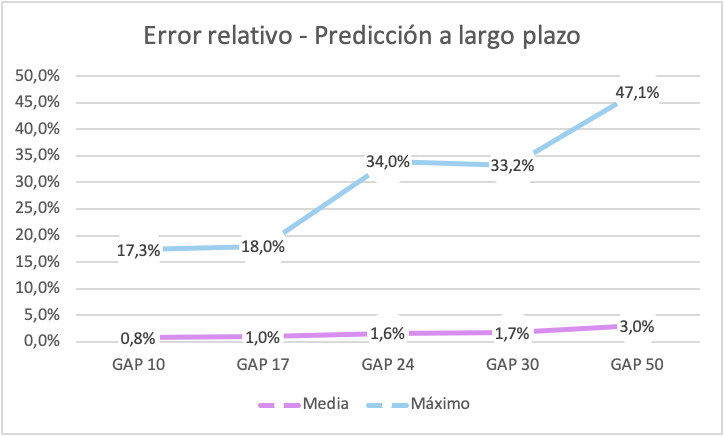
\includegraphics[width=0.7\textwidth]{ figures/test_mod/REC/complex/largoplazo.png}
			\caption{Comparación del error relativo al aumentar el \textit{gap}~(Combinada, 10000 muestras de \textit{test})}
			\label{fig.gap}
		\end{center}
\end{figure}
\vspace{-10pt}

A la vista de estos resultados queda patente el hecho de que poner la vista en una posición más lejana en el tiempo complica la tarea de predicción de la red. A medida que se aumenta la separación temporal entre el último elemento conocido y el que se quiere estimar la relación entre ambas se va difuminando, perdiendo la capacidad de predicción progresivamente. Sin embargo, esta pérdida se realiza siempre en umbrales admisibles: en una imagen de 640x480, por ejemplo, se obtienen 14 píxeles de media de error a 30 fotogramas (1.7\%) y 24 a 50 fotogramas (3\%).

\subsection{Resumen de resultados}
En la Tabla~\ref{tab.lstm4} se muestra el resumen de los resultados obtenidos en las distintas dinámicas consideradas para la red \textit{LSTM-4}.
\begin{table}[H]
	\centering
	\begin{tabular}{{|l|c|c|}}
		\hline
		\multicolumn{2}{|c|}{\textbf{Dinámica}} & \textbf{LSTM-4}\\ \hline 
		\multicolumn{1}{|c|}{Lineal}
        &2~\acrshort{dof} & \cellcolor{darkgreen}0.12\%\\ 
        \hline
        \multicolumn{1}{|c|}{Parabólica}
        &3~\acrshort{dof} & \cellcolor{darkgreen}0.5\%\\ 
        \hline
        \multicolumn{1}{|c|}{Sinusoidal}
        &4~\acrshort{dof} & \cellcolor{greenyellow}0.61\%\\
        \hline
        \multicolumn{2}{|c|}{Combinada} & \cellcolor{greenyellow}0.81\%\\ \hline 
	\end{tabular}
	\caption{Promedio del error relativo en \textit{test} al evaluar la red LSTM-4 con imágenes modeladas y distintas dinámicas (10000 muestras de \textit{test}).}
	\label{tab.lstm4}
\end{table}

Como anteriormente,se han evaluado todas las redes con un conjunto de 10000 muestras para que la comparación entre ellas sea equitativa.

\section{Comparativa global} \label{sec.comp_mod}
Tras realizar los experimentos con imágenes modeladas se obtiene un conjunto de redes entrenadas para las distintas dinámicas. Con el objetivo de compararlas de una forma rápida, se ha elaborado la Tabla~\ref{tab.comp_mod}. Esta tabla sigue el mismo código de colores especificado en el Apartado~\ref{ap.resumen_RNNmlp}, añadiendo el gris para aquellos experimentos que no han sido considerados. Además, el valor numérico asociado, promedio del error relativo, ilustra de una forma cuantitativa las prestaciones obtenidas, aunque no es la única figura de mérito utilizada para la asignación del color en la celda. También se han evaluado todas las redes con un conjunto de 10000 muestras para una comparación equitativa.

\begin{table}[H]
	\centering
	\begin{tabular}{{|l|c|c|c|c|}}
		\hline
		\multicolumn{2}{|c|}{\textbf{Dinámica}} & \textbf{\acrshort{mlp}} & \textbf{LSTM-1} & \textbf{LSTM-4}\\ \hline 
		\multirow{2}{*}{Lineal}
		&1~\acrshort{dof} & \cellcolor{darkgreen}0.21\% & \cellcolor{darkgreen}0.16\% & \cellcolor{gray!30}\\
		\cline{2-5}
        &2~\acrshort{dof} & \cellcolor{darkgreen}0.31\% & \cellcolor{darkgreen}0.25\% & \cellcolor{darkgreen}0.12\% \\ 
        \hline
        \multirow{3}{*}{Parabólica}
        &1~\acrshort{dof} & \cellcolor{darkgreen}0.28\% & \cellcolor{darkgreen}0.12\% & \cellcolor{gray!30}\\
		\cline{2-5}
        &2~\acrshort{dof} & \cellcolor{darkgreen}0.42\% & \cellcolor{darkgreen}0.35\% & \cellcolor{gray!30}\\
        \cline{2-5}
        &3~\acrshort{dof} & \cellcolor{darkgreen}0.65\%& \cellcolor{darkgreen}0.58\%& \cellcolor{darkgreen}0.6\%\\ 
        \hline
        \multirow{4}{*}{Sinusoidal}
        &1~\acrshort{dof} & \cellcolor{darkgreen}0.54\% & \cellcolor{darkgreen}0.42\% & \cellcolor{gray!30} \\
        \cline{2-5}
        &2~\acrshort{dof} & \cellcolor{myorange}3.89\% & \cellcolor{greenyellow}0.89\% & \cellcolor{gray!30} \\
        \cline{2-5}
        &3~\acrshort{dof} & \cellcolor{gray!30} & \cellcolor{greenyellow}0.84\% & \cellcolor{gray!30} \\
        \cline{2-5}
        &4~\acrshort{dof} & \cellcolor{gray!30} & \cellcolor{myorange} 4.09\%& \cellcolor{greenyellow}0.61\%\\ 
        \hline
        \multicolumn{2}{|c|}{Combinada} & \cellcolor{gray!30} & \cellcolor{gray!30} & \cellcolor{greenyellow}0.81\%\\ \hline 
	\end{tabular}
	\caption{Comparativa del promedio de error relativo en las distintas redes para imágenes modeladas con las distintas dinámicas (10000 muestras de \textit{test}).}
	\label{tab.comp_mod}
\end{table}

Se puede observar que la red que mejores resultados aporta es la \textit{LSTM-4}, que es capaz de realizar una predicción razonable en todas las dinámicas consideradas. Además, se refleja que el uso de la recurrencia aporta una mejora en la calidad de la predicción y que el aumento de capas recurrentes hace que se lleguen a dominar todas las dinámicas en su grado más complejo.
